\newcommand{\mypapersize}{A4}
%% e.g., "A4", "letter", "legal", "executive", ...
%% The size of the paper of the resulting PDF file.
\newcommand{\mylaterality}{oneside}
%% "oneside" or "twoside"
%% Either you are creating a document which is printed on both, left pages
%% and right pages (twoside) or you create a document which is printed
%% on right pages only (oneside).

\newcommand{\mydraft}{false}
%% "true" or "false"
%% Use draft mode? If true, included graphics are replaced by empty
%% rectangles (of same size) and overfull boxes (in margin space) are
%% marked with black box (-> easy to spot!)

\newcommand{\myparskip}{half}
%% e.g., "no", "full", "half", ...
%% How to separate paragraphs: indention ("no") or spacing ("half",
%% "full", ...).

\newcommand{\myBCOR}{0mm}
%% Inner binding correction. This value depends on the method which is
%% being used to bind your printed result. Some techniques do not
%% require a binding correction at all ("0mm"), other require for
%% example "5mm". Refer to KOMA script documentation for a detailed
%% explanation what a binding correction is and how to measure it.

\newcommand{\myfontsize}{12pt}
%% e.g., 10pt, 11pt, 12pt
%% The font size of the main text in pt (points).

\newcommand{\mylinespread}{1.0}
%% e.g., 1.0, 1.5, 2.0
%% Line spacing in %/100. For example 1.5 means 150% of the usual line
%% spacing. Please use with caution: 100% ("1.0") is fine because the
%% font was designed for it.

\newcommand{\mylanguage}{spanish}
%% "english,ngerman", "ngerman,english", ...
%% NOTE: The *last* language is the active one!
%% See babel documentation for further details.

%% BibLaTeX-settings: (see biblatex reference for further description)
\newcommand{\mybiblatexstyle}{authoryear}
%% e.g., "alphabetic", "authoryear", ...
%% The biblatex style which is being used for referencing. See
%% biblatex documentation for further details and more values.
%%
%% CAUTION: if you change the style, please check for (in)compatible
%%          "biblatex" package options in the file
%%          "template/preamble.tex"! For example: "alphabetic" does
%%          not have an option "dashed=..." and causes an error if it
%%          does not get removed from the list of options.

\newcommand{\mybiblatexdashed}{false}  %% "true" or "false"
%% If true: replace recurring reference authors with a dash.

\newcommand{\mybiblatexbackref}{true}  %% "true" or "false"
%% If true: create backward links from reference to citations.

\newcommand{\mybiblatexfile}{references-biblatex.bib}
%% Name of the biblatex file that holds the references.

\newcommand{\mydispositioncolor}{30,103,182}
%% e.g., "30,103,182" (blue/turquois), "0,0,0" (black), ...
%% Color of the headings and so forth in RGB (red,green,blue) values.
%% NOTE: if you are using "0,0,0" for black, printers might still
%%       recognize pages as color pages. In case this is a problem
%%       (paying for color print-outs vs. paying for b/w-printouts)
%%       please edit file "template/preamble.tex" and change
%%       "\definecolor{DispositionColor}{RGB}{\mydispositioncolor}"
%%       to "\definecolor{DispositionColor}{gray}{0}" and thus
%%       overwriting the value of \mydispositioncolor above.

\newcommand{\mycolorlinks}{true}  %% "true" or "false"
%% Enables or disables colored links (hyperref package).

\newcommand{\mytitlepage}{template/title_Thesis_TU_Graz}
%% Your own or one of following pre-defined title pages:
%% "template/title_plain_maketitle": simple maketitle page
%% "template/title_Diplomarbeit_KF_Uni_Graz.tex": fancy (german) title page for KF Uni Graz
%% "template/title_Thesis_TU_Graz":
%%             titlepage for Graz University of Technology (correct
%%             (old?) Corporate Design) by Karl Voit (2012)
%% "template/title_Thesis_TU_Graz_-_kazemakase":
%%             titlepage for Graz University of Technology
%%             (correct new Corporate Design) by kazemakase (2013):
%%             see https://github.com/novoid/LaTeX-KOMA-template/issues/5
%% "template/title_VWA": titlepage for Vorwissenschaftliche Arbeit

\newcommand{\mytodonotesoptions}{}
%% e.g., "" (empty), "disable", ...
%% Options for the todonotes-package. If "disable", all todonotes will
%% be hidden (including listoftodos).

%% Load main settings for document preamble:
\documentclass[%
fontsize=\myfontsize,%% size of the main text
paper=\mypapersize,  %% paper format
parskip=\myparskip,  %% vertical space between paragraphs (instead of indenting first par-line)
DIV=calc,            %% calculates a good DIV value for type area; 66 characters/line is great
headinclude=true,    %% is header part of margin space or part of page content?
footinclude=false,   %% is footer part of margin space or part of page content?
open=right,          %% "right" or "left": start new chapter on right or left page
appendixprefix=true, %% adds appendix prefix; only for book-classes with \backmatter
bibliography=totoc,  %% adds the bibliography to table of contents (without number)
draft=\mydraft,      %% if true: included graphics are omitted and black boxes
                     %%          mark overfull boxes in margin space
BCOR=\myBCOR,        %% binding correction (depends on how you bind
                     %% the resulting printout.
\mylaterality        %% oneside: document is not printed on left and right sides, only right side
                     %% twoside: document is printed on left and right sides
]{scrbook}  %% article class of KOMA: "scrartcl", "scrreprt", or "scrbook".
            %% CAUTION: If documentclass will be changed, *many* other things
            %%          change as well like heading structure, ...

\usepackage[utf8]{inputenc} %% UTF8 as input characters
\usepackage[\mylanguage]{babel}  %% used languages; default language is *last*
\usepackage{scrpage2} %%  advanced page style using KOMA
\usepackage[backend=biber, %% using "biber" to compile references (instead of "biblatex")
style=\mybiblatexstyle, %% see biblatex documentation
%style=alphabetic, %% see biblatex documentation
% dashed=\mybiblatexdashed, %% do *not* replace recurring reference authors with a dash
% backref=\mybiblatexbackref, %% create backlings from references to citations
% natbib=true, %% offering natbib-compatible commands
hyperref=true, %% using hyperref-package references
]{biblatex}  %% remove, if using BibTeX instead of biblatex

\addbibresource{\mybiblatexfile} %% remove, if using BibTeX instead of biblatex

\ifthenelse{\boolean{\mydraft}}{   %% the \mydraft switches between
                                   %% showing rectangles instead of graphics
  \usepackage[pdftex,draft]{graphicx}
}
{
  \usepackage[pdftex]{graphicx}
}

\usepackage{pifont}

\usepackage{ifthen}

\newboolean{myaddcolophon}
\newboolean{myaddlistoftodos}
\newboolean{english_affidavit}

\usepackage{xspace}
\usepackage[usenames,dvipsnames]{xcolor}
\definecolor{DispositionColor}{RGB}{\mydispositioncolor} %% used for links and so forth in screen-version

\usepackage[normalem]{ulem}
\usepackage{framed}
\usepackage{eso-pic}
\usepackage{enumitem}
\usepackage[\mytodonotesoptions]{todonotes}  %% option "disable" removes all todonotes output from resulting document
\usepackage{units}
%% DO NOT REMOVE THIS LINE!
\usepackage{subcaption}
\usepackage{amsmath}
\setboolean{myaddcolophon}{false}  %% "true" or "false"
%% If set to "true": a colophon (with notes about this document
%% template, LaTeX, ...) is added after the title page.
%% Please do not set to "false" without a good reason. The colophon
%% helps your readers to get in touch with LaTeX and to find this template.

\setboolean{myaddlistoftodos}{false}  %% "true" or "false"
%% If set to "true": the current list of open todos is added after the
%% table of contents. If \mytodonotesoptions is set to "disable", no
%% list of todos is added, independent of this setting here.

\setboolean{english_affidavit}{false}  %% "true" or "false"
%% If set to "true": the language of the statutory declaration text is set to
%% English, otherwise it is in German.


%% ========================================================================
%%%% Document metadata
%% ========================================================================

%% general metadata:
\newcommand{\myauthor}{César Bolívar Severino}  %% also used for PDF metadata (hyperref)
\newcommand{\myauthorwithexistingtitles}{\myauthor{}, OLDDEGREE}  %% including
                                %% university degree already held
                                %% (BSc, MSc, ...)
\newcommand{\mytitle}{Resolviendo el cubo de Rubik con el robot Baxter}  %% also used for PDF metadata (hyperref)
\newcommand{\mysubtitle}{ }  %% only used with title_Thesis_TU_Graz_-_kazemakase
\newcommand{\mysubject}{SUBJECT}  %% also used for PDF metadata (hyperref)
\newcommand{\mykeywords}{KEYWORDS}  %% also used for PDF metadata (hyperref)

%% this information is used only for generating the title page:
\newcommand{\myworktitle}{Memoria de Título}  %% official type of work like ``Master theses''
\newcommand{\mygrade}{Ingeniero Civil Informático} %% title you are getting with this work like ``Master of ...''
\newcommand{\mystudy}{Ingeniería Civil Informática} %% your study like ``Arts''
\newcommand{\mydegreeprogramme}{Programa: \mystudy} %% Master's or PhD degree programme
\newcommand{\myuniversity}{Universidad de Concepción} %% your university/school
\newcommand{\myfaculty}{Facultad de Ingeniería}  %% only used with title_Thesis_TU_Graz_-_kazemakase
\newcommand{\myinstitute}{Departamento de Ingeniería Informática y Ciencias de la Computación} %% affiliation
\newcommand{\myinstitutehead}{Univ.-Prof.\,Dipl-Ing.\,Dr.techn.~Some One} %% head of institute
\newcommand{\mysupervisor}{Julio Godoy del Campo} %% your supervisor
\newcommand{\mycosupervisor}{\ }  %% only used with title_Thesis_TU_Graz_-_kazemakase
\newcommand{\myevaluator}{Roberto Asín Achá, Eduardo Méndez Ortiz} %% your evaluator
\newcommand{\myhomestreet}{Street~42} %% your home street (with house number)
\newcommand{\myhometown}{Graz} %% your home town
\newcommand{\myhomepostalnumber}{8010} %% your postal number of home town
\newcommand{\mysubmissionmonth}{November} %% month you are handing in
\newcommand{\mysubmissionyear}{2019} %% year you are handing in
\newcommand{\mysubmissiontown}{\myhometown} %% town of handing in (or \myhometown)


%% additional information for generic_documentation title page
\newcommand{\myid}{1234567} %% Matrikelnummer
\newcommand{\mylecture}{LECTURE} %%

%%%% MISC command definitions
%% Time-stamp: <2015-04-30 17:19:58 vk>
%%%% === Disclaimer: =======================================================
%% created by
%%
%%      Karl Voit
%%
%% using GNU/Linux, GNU Emacs & LaTeX 2e
%%

%doc%
%doc% \section{\texttt{mycommands.tex} --- various definitions}\myinteresting
%doc% \label{sec:mycommands}
%doc%
%doc% In file \verb#template/mycommands.tex# many useful commands are being
%doc% defined. 
%doc% 
%doc% \paragraph{What should I do with this file?} Please take a look at its 
%doc% content to get the most out of your document.
%doc% 

%doc% 
%doc% One of the best advantages of \LaTeX{} compared to \myacro{WYSIWYG} software products is
%doc% the possibility to define and use macros within text. This empowers the user to
%doc% a great extend.  Many things can be defined using \verb#\newcommand{}# and
%doc% automates repeating tasks. It is recommended to use macros not only for
%doc% repetitive tasks but also for separating form from content such as \myacro{CSS}
%doc% does for \myacro{XHTML}. Think of including graphics in your document: after
%doc% writing your book, you might want to change all captions to the upper side of
%doc% each figure. In this case you either have to modify all
%doc% \texttt{includegraphics} commands or you were clever enough to define something
%doc% like \verb#\myfig#\footnote{See below for a detailed description}. Using a
%doc% macro for including graphics enables you to modify the position caption on only
%doc% \emph{one} place: at the definition of the macro.
%doc% 
%doc% The following section describes some macros that came with this document template
%doc% from \myLaT and you are welcome to modify or extend them or to create
%doc% your own macros!
%doc% 

%doc% 
%doc% \subsection{\texttt{myfig} --- including graphics made easy}
%doc% 
%doc% The classic: you can easily add graphics to your document with \verb#\myfig#:
%doc% \begin{verbatim}
%doc%  \myfig{flower}%% filename w/o extension in the folder figures
%doc%        {width=0.7\textwidth}%% maximum width/height, aspect ratio will be kept
%doc%        {This flower was photographed at my home town in 2010}%% caption
%doc%        {Home town flower}%% optional (short) caption for list of figures
%doc%        {fig:flower}%% label
%doc% \end{verbatim}
%doc% 
%doc% There are many advantages of this command (compared to manual
%doc% \texttt{figure} environments and \texttt{includegraphics} commands:
%doc% \begin{itemize}
%doc% \item consistent style throughout the whole document
%doc% \item easy to change; for example move caption on top
%doc% \item much less characters to type (faster, error prone)
%doc% \item less visual clutter in the \TeX{}-files
%doc% \end{itemize}
%doc% 
%doc% 
\newcommand{\myfig}[5]{
%% example:
% \myfig{}%% filename in figures folder
%       {width=0.5\textwidth,height=0.5\textheight}%% maximum width/height, aspect ratio will be kept
%       {}%% caption
%       {}%% optional (short) caption for list of figures
%       {}%% label
\begin{figure}%[htp]
  \centering
  \includegraphics[keepaspectratio,#2]{figures/#1}
  \caption[#4]{#3}
  \label{#5} %% NOTE: always label *after* caption!
\end{figure}
}


%doc% 
%doc% \subsection{\texttt{myclone} --- repeat things!}
%doc% 
%doc% Using \verb#\myclone[42]{foobar}# results the text \enquote{foobar} printed 42 times.
%doc% But you can not only repeat text output with \texttt{myclone}. 
%doc%
%doc% Default argument
%doc% for the optional parameter \enquote{number of times} (like \enquote{42} in the example above) 
%doc% is set to two.
%doc% 
%% \myclone[x]{text}
\newcounter{myclonecnt}
\newcommand{\myclone}[2][2]{%
  \setcounter{myclonecnt}{#1}%
  \whiledo{\value{myclonecnt}>0}{#2\addtocounter{myclonecnt}{-1}}%
}

%old% %d oc% 
%old% %d oc% \subsection{\texttt{fixxme} --- sidemark something as unfinished}
%old% %d oc% 
%old% %d oc% You know it: something has to be fixed and you can not do it right
%old% %d oc% now. In order to \texttt{not} forget about it, you might want to add a
%old% %d oc% note like \verb+\fixxme{check again}+ which inserts a note on the page
%old% %d oc% margin such as this\fixxme{check again} example.
%old% %d oc%
%old% \newcommand{\fixxme}[1]{%%
%old% \textcolor{red}{FIXXME}\marginpar{\textcolor{red}{#1}}%%
%old% }


%%%% End 
%%% Local Variables:
%%% mode: latex
%%% mode: auto-fill
%%% mode: flyspell
%%% eval: (ispell-change-dictionary "en_US")
%%% TeX-master: "../main"
%%% End:
%% vim:foldmethod=expr
%% vim:fde=getline(v\:lnum)=~'^%%%%'?0\:getline(v\:lnum)=~'^%doc.*\ .\\%(sub\\)\\?section{.\\+'?'>1'\:'1':


%%%% Typographic settings
%%%% Time-stamp: <2015-08-22 17:20:32 vk>
%%%% === Disclaimer: =======================================================
%% created by
%%
%%      Karl Voit
%%
%% using GNU/Linux, GNU Emacs & LaTeX 2e
%%
%doc%
%doc% \section{\texttt{typographic\_settings.tex} --- Typographic finetuning}
%doc%
%doc% The settings of file \verb#template/typographic_settings.tex# contain
%doc% typographic finetuning related to things mentioned in literature.  The
%doc% settings in this file relates to personal taste and most of all: 
%doc% \emph{typographic experience}. 
%doc% 
%doc% \paragraph{What should I do with this file?} You might as well skip the whole
%doc% file by excluding the \verb#%%%% Time-stamp: <2015-08-22 17:20:32 vk>
%%%% === Disclaimer: =======================================================
%% created by
%%
%%      Karl Voit
%%
%% using GNU/Linux, GNU Emacs & LaTeX 2e
%%
%doc%
%doc% \section{\texttt{typographic\_settings.tex} --- Typographic finetuning}
%doc%
%doc% The settings of file \verb#template/typographic_settings.tex# contain
%doc% typographic finetuning related to things mentioned in literature.  The
%doc% settings in this file relates to personal taste and most of all: 
%doc% \emph{typographic experience}. 
%doc% 
%doc% \paragraph{What should I do with this file?} You might as well skip the whole
%doc% file by excluding the \verb#%%%% Time-stamp: <2015-08-22 17:20:32 vk>
%%%% === Disclaimer: =======================================================
%% created by
%%
%%      Karl Voit
%%
%% using GNU/Linux, GNU Emacs & LaTeX 2e
%%
%doc%
%doc% \section{\texttt{typographic\_settings.tex} --- Typographic finetuning}
%doc%
%doc% The settings of file \verb#template/typographic_settings.tex# contain
%doc% typographic finetuning related to things mentioned in literature.  The
%doc% settings in this file relates to personal taste and most of all: 
%doc% \emph{typographic experience}. 
%doc% 
%doc% \paragraph{What should I do with this file?} You might as well skip the whole
%doc% file by excluding the \verb#\input{template/typographic_settings.tex}# command
%doc% in \texttt{main.tex}.  For standard usage it is recommended to stay with the
%doc% default settings.
%doc% 
%doc% 
%% ========================================================================

%doc%
%doc% Some basic microtypographic settings are provided by the
%doc% \texttt{microtype}
%doc% package\footnote{\url{http://ctan.org/pkg/microtype}}. This template
%doc% uses the rather conservative package parameters: \texttt{protrusion=true,factor=900}.
\usepackage[protrusion=true,factor=900]{microtype}

%doc%
%doc% \subsection{French spacing}
%doc%
%doc% \paragraph{Why?} see~\textcite[p.\,28, p.\,30]{Bringhurst1993}: `2.1.4 Use a single word space between sentences.'
%doc%
%doc% \paragraph{How?} see~\textcite[p.\,185]{Eijkhout2008}:\\
%doc% \verb#\frenchspacing  %% Macro to switch off extra space after punctuation.# \\
\frenchspacing  %% Macro to switch off extra space after punctuation.
%doc%
%doc% Note: This setting might be default for \myacro{KOMA} script.
%doc%


%doc%
%doc% \subsection{Font}
%doc% 
%doc% This template is using the Palatino font (package \texttt{mathpazo}) which results
%doc% in a legible document and matching mathematical fonts for printout.
%doc% 
%doc% It is highly recommended that you either stick to the Palatino font or use the
%doc% \LaTeX{} default fonts (by removing the package \texttt{mathpazo}).
%doc% 
%doc% Chosing different fonts is not
%doc% an easy task. Please leave this to people with good knowledge on this subject.
%doc% 
%doc% One valid reason to change the default fonts is when your document is mainly
%doc% read on a computer screen. In this case it is recommended to switch to a font
%doc% \textsf{which is sans-serif like this}. This template contains several alternative
%doc% font packages which can be activated in this file.
%doc% 

% for changing the default font, please go to the next subsection!

%doc%
%doc% \subsection{Text figures}
%doc% 
%doc% \ldots also called old style numbers such as 0123456789. 
%doc% (German: \enquote{Mediäval\-ziffern\footnote{\url{https://secure.wikimedia.org/wikibooks/de/wiki/LaTeX-W\%C3\%B6rterbuch:\_Medi\%C3\%A4valziffern}}})
%doc% \paragraph{Why?} see~\textcite[p.\,44f]{Bringhurst1993}: 
%doc% \begin{quote}
%doc% `3.2.1 If the font includes both text figures and titling figures, use
%doc%  titling figures only with full caps, and text figures in all other
%doc%  circumstances.'
%doc% \end{quote}
%doc% 
%doc% \paragraph{How?} 
%doc% Quoted from Wikibooks\footnote{\url{https://secure.wikimedia.org/wikibooks/en/wiki/LaTeX/Formatting\#Text\_figures\_.28.22old\_style.22\_numerals.29}}:
%doc% \begin{quote}
%doc% Some fonts do not have text figures built in; the textcomp package attempts to
%doc% remedy this by effectively generating text figures from the currently-selected
%doc% font. Put \verb#\usepackage{textcomp}# in your preamble. textcomp also allows you to
%doc% use decimal points, properly formatted dollar signs, etc. within
%doc% \verb#\oldstylenums{}#.
%doc% \end{quote}
%doc% \ldots but proposed \LaTeX{} method does not work out well. Instead use:\\
%doc% \verb#\usepackage{hfoldsty}#  (enables text figures using additional font) or \\
%doc% \verb#\usepackage[sc,osf]{mathpazo}# (switches to Palatino font with small caps and old style figures enabled).
%doc%
%\usepackage{hfoldsty}  %% enables text figures using additional font
%% ... OR use ...
\usepackage[sc,osf]{mathpazo} %% switches to Palatino with small caps and old style figures

%% Font selection from:
%%     http://www.matthiaspospiech.de/latex/vorlagen/allgemein/preambel/fonts/
%% use following lines *instead* of the mathpazo package above:
%% ===== Serif =========================================================
%% for Computer Modern (LaTeX default font), simply remove the mathpazo above
%\usepackage{charter}\linespread{1.05} %% Charter
%\usepackage{bookman}                  %% Bookman (laedt Avant Garde !!)
%\usepackage{newcent}                  %% New Century Schoolbook (laedt Avant Garde !!)
%% ===== Sans Serif ====================================================
%\renewcommand{\familydefault}{\sfdefault}  %% this one in *combination* with the default mathpazo package
%\usepackage{cmbright}                  %% CM-Bright (eigntlich eine Familie)
%\usepackage{tpslifonts}                %% tpslifonts % Font for Slides


%doc% 
%doc% \subsection{\texttt{myacro} --- Abbrevations using \textsc{small caps}}\myinteresting
%doc% \label{sec:myacro}
%doc% 
%doc% \paragraph{Why?} see~\textcite[p.\,45f]{Bringhurst1993}: `3.2.2 For abbrevations and
%doc% acronyms in the midst of normal text, use spaced small caps.'
%doc% 
%doc% \paragraph{How?} Using the predefined macro \verb#\myacro{}# for things like
%doc% \myacro{UNO} or \myacro{UNESCO} using \verb#\myacro{UNO}# or \verb#\myacro{UNESCO}#.
%doc% 
\DeclareRobustCommand{\myacro}[1]{\textsc{\lowercase{#1}}} %%  abbrevations using small caps


%doc% 
%doc% \subsection{Colorized headings and links}
%doc% 
%doc% This document template is able to generate an output that uses colorized
%doc% headings, captions, page numbers, and links. The color named `DispositionColor'
%doc% used in this document is defined near the definition of package \texttt{color}
%doc% in the preamble (see section~\ref{subsec:miscpackages}). The changes required
%doc% for headings, page numbers, and captions are defined here.
%doc% 
%doc% Settings for colored links are handled by the definitions of the
%doc% \texttt{hyperref} package (see section~\ref{sec:pdf}).
%doc% 
\setheadsepline{.4pt}[\color{DispositionColor}]
\renewcommand{\headfont}{\normalfont\sffamily\color{DispositionColor}}
\renewcommand{\pnumfont}{\normalfont\sffamily\color{DispositionColor}}
\addtokomafont{disposition}{\color{DispositionColor}}
\addtokomafont{caption}{\color{DispositionColor}\footnotesize}
\addtokomafont{captionlabel}{\color{DispositionColor}}

%doc% 
%doc% \subsection{No figures or tables below footnotes}
%doc% 
%doc% \LaTeX{} places floating environments below footnotes if \texttt{b}
%doc% (bottom) is used as (default) placement algorithm. This is certainly
%doc% not appealing for most people and is deactivated in this template by
%doc% using the package \texttt{footmisc} with its option \texttt{bottom}.
%doc% 
%% see also: http://www.komascript.de/node/858 (German description)
\usepackage[bottom]{footmisc}

%doc% 
%doc% \subsection{Spacings of list environments}
%doc% 
%doc% By default, \LaTeX{} is using vertical spaces between items of enumerate, 
%doc% itemize and description environments. This is fine for multi-line items.
%doc% Many times, the user does just write single-line items where the larger
%doc% vertical space is inappropriate. The \href{http://ctan.org/pkg/enumitem}{enumitem}
%doc% package provides replacements for the pre-defined list environments and
%doc% offers many options to modify their appearances.
%doc% This template is using the package option for \texttt{noitemsep} which
%doc% mimimizes the vertical space between list items.
%doc% 
\usepackage{enumitem}
\setlist{noitemsep}   %% kills the space between items

%doc% 
%doc% \subsection{\texttt{csquotes} --- Correct quotation marks}\myinteresting
%doc% \label{sub:csquotes}
%doc% 
%doc% \emph{Never} use quotation marks found on your keyboard.
%doc% They end up in strange characters or false looking quotation marks.
%doc% 
%doc% In \LaTeX{} you are able to use typographically correct quotation marks. The package 
%doc% \href{http://www.ctan.org/pkg/csquotes}{\texttt{csquotes}} offers you with 
%doc% \verb#\enquote{foobar}# a command to get correct quotation marks around \enquote{foobar}.
%doc% Please do check the package options in order to modify
%doc% its settings according to the language used\footnote{most of the time in 
%doc% combination with the language set in the options of the \texttt{babel} package}.
%doc% 
%doc% \href{http://www.ctan.org/pkg/csquotes}{\texttt{csquotes}} is also recommended 
%doc% by \texttt{biblatex} (see Section~\ref{sec:references}). 
\usepackage[babel=true,strict=true,english=american,german=guillemets]{csquotes}

%doc% 
%doc% \subsection{Line spread}
%doc% 
%doc% If you have to enlarge the distance between two lines of text, you can
%doc% increase it using the \texttt{\mylinespread} command in \texttt{main.tex}. By default, it is
%doc% deactivated (set to 100~percent). Modify only with caution since it influences the
%doc% page layout and could lead to ugly looking documents.
\linespread{\mylinespread}

%doc% 
%doc% \subsection{Optional: Lines above and below the chapter head}
%doc% 
%doc% This is not quite something typographic but rather a matter of taste.
%doc% \myacro{KOMA} Script offers \href{http://www.komascript.de/node/24}{a method to
%doc% add lines above and below chapter head} which is disabled by
%doc% default. If you want to enable this feature, remove corresponding
%doc% comment characters from the settings.
%doc% 
%% Source: http://www.komascript.de/node/24
%disabled% %% 1st get a new command
%disabled% \newcommand*{\ORIGchapterheadstartvskip}{}%
%disabled% %% 2nd save the original definition to the new command
%disabled% \let\ORIGchapterheadstartvskip=\chapterheadstartvskip
%disabled% %% 3rd redefine the command using the saved original command
%disabled% \renewcommand*{\chapterheadstartvskip}{%
%disabled%   \ORIGchapterheadstartvskip
%disabled%   {%
%disabled%     \setlength{\parskip}{0pt}%
%disabled%     \noindent\color{DispositionColor}\rule[.3\baselineskip]{\linewidth}{1pt}\par
%disabled%   }%
%disabled% }
%disabled% %% see above
%disabled% \newcommand*{\ORIGchapterheadendvskip}{}%
%disabled% \let\ORIGchapterheadendvskip=\chapterheadendvskip
%disabled% \renewcommand*{\chapterheadendvskip}{%
%disabled%   {%
%disabled%     \setlength{\parskip}{0pt}%
%disabled%     \noindent\color{DispositionColor}\rule[.3\baselineskip]{\linewidth}{1pt}\par
%disabled%   }%
%disabled%   \ORIGchapterheadendvskip
%disabled% }

%doc% 
%doc% \subsection{Optional: Chapter thumbs}
%doc% 
%doc% This is not quite something typographic but rather a matter of taste.
%doc% \myacro{KOMA} Script offers \href{http://www.komascript.de/chapterthumbs-example}{a method to
%doc% add chapter thumbs} (in combination with the package \texttt{scrpage2}) which is disabled by
%doc% default. If you want to enable this feature, remove corresponding
%doc% comment characters from the settings.
%doc% 
%disabled% \makeatletter
%disabled% % Safty first
%disabled% \@ifundefined{chapter}{\let\chapter\undefined
%disabled%   \chapter must be defined to use chapter thumbs!}{%
%disabled%  
%disabled% % Two new commands for the width and height of the boxes with the
%disabled% % chapter number at the thumbs (use of commands instead of lengths
%disabled% % for sparing registers)
%disabled% \newcommand*{\chapterthumbwidth}{2em}
%disabled% \newcommand*{\chapterthumbheight}{1em}
%disabled%  
%disabled% % Two new commands for the colors of the box background and the
%disabled% % chapter numbers of the thumbs
%disabled% \newcommand*{\chapterthumbboxcolor}{black}
%disabled% \newcommand*{\chapterthumbtextcolor}{white}
%disabled%  
%disabled% % New command to set a chapter thumb. I'm using a group at this
%disabled% % command, because I'm changing the temporary dimension \@tempdima
%disabled% \newcommand*{\putchapterthumb}{%
%disabled%   \begingroup
%disabled%     \Large
%disabled%     % calculate the horizontal possition of the right paper border
%disabled%     % (I ignore \hoffset, because I interprete \hoffset moves the page
%disabled%     % at the paper e.g. if you are using cropmarks)
%disabled%     \setlength{\@tempdima}{\@oddheadshift}% (internal from scrpage2)
%disabled%     \setlength{\@tempdima}{-\@tempdima}%
%disabled%     \addtolength{\@tempdima}{\paperwidth}%
%disabled%     \addtolength{\@tempdima}{-\oddsidemargin}%
%disabled%     \addtolength{\@tempdima}{-1in}%
%disabled%     % putting the thumbs should not change the horizontal
%disabled%     % possition
%disabled%     \rlap{%
%disabled%       % move to the calculated horizontal possition
%disabled%       \hspace*{\@tempdima}%
%disabled%       % putting the thumbs should not change the vertical
%disabled%       % possition
%disabled%       \vbox to 0pt{%
%disabled%         % calculate the vertical possition of the thumbs (I ignore
%disabled%         % \voffset for the same reasons told above)
%disabled%         \setlength{\@tempdima}{\chapterthumbwidth}%
%disabled%         \multiply\@tempdima by\value{chapter}%
%disabled%         \addtolength{\@tempdima}{-\chapterthumbwidth}%
%disabled%         \addtolength{\@tempdima}{-\baselineskip}%
%disabled%         % move to the calculated vertical possition
%disabled%         \vspace*{\@tempdima}%
%disabled%         % put the thumbs left so the current horizontal possition
%disabled%         \llap{%
%disabled%           % and rotate them
%disabled%           \rotatebox{90}{\colorbox{\chapterthumbboxcolor}{%
%disabled%               \parbox[c][\chapterthumbheight][c]{\chapterthumbwidth}{%
%disabled%                 \centering
%disabled%                 \textcolor{\chapterthumbtextcolor}{%
%disabled%                   \strut\thechapter}\\
%disabled%               }%
%disabled%             }%
%disabled%           }%
%disabled%         }%
%disabled%         % avoid overfull \vbox messages
%disabled%         \vss
%disabled%       }%
%disabled%     }%
%disabled%   \endgroup
%disabled% }
%disabled%  
%disabled% % New command, which works like \lohead but also puts the thumbs (you
%disabled% % cannot use \ihead with this definition but you may change this, if
%disabled% % you use more internal scrpage2 commands)
%disabled% \newcommand*{\loheadwithchapterthumbs}[2][]{%
%disabled%   \lohead[\putchapterthumb#1]{\putchapterthumb#2}%
%disabled% }
%disabled%  
%disabled% % initial use
%disabled% \loheadwithchapterthumbs{}
%disabled% \pagestyle{scrheadings}
%disabled%  
%disabled% }
%disabled% \makeatother

%%%% END
%%% Local Variables:
%%% mode: latex
%%% mode: auto-fill
%%% mode: flyspell
%%% eval: (ispell-change-dictionary "en_US")
%%% TeX-master: "../main"
%%% End:
%% vim:foldmethod=expr
%% vim:fde=getline(v\:lnum)=~'^%%%%'?0\:getline(v\:lnum)=~'^%doc.*\ .\\%(sub\\)\\?section{.\\+'?'>1'\:'1':
# command
%doc% in \texttt{main.tex}.  For standard usage it is recommended to stay with the
%doc% default settings.
%doc% 
%doc% 
%% ========================================================================

%doc%
%doc% Some basic microtypographic settings are provided by the
%doc% \texttt{microtype}
%doc% package\footnote{\url{http://ctan.org/pkg/microtype}}. This template
%doc% uses the rather conservative package parameters: \texttt{protrusion=true,factor=900}.
\usepackage[protrusion=true,factor=900]{microtype}

%doc%
%doc% \subsection{French spacing}
%doc%
%doc% \paragraph{Why?} see~\textcite[p.\,28, p.\,30]{Bringhurst1993}: `2.1.4 Use a single word space between sentences.'
%doc%
%doc% \paragraph{How?} see~\textcite[p.\,185]{Eijkhout2008}:\\
%doc% \verb#\frenchspacing  %% Macro to switch off extra space after punctuation.# \\
\frenchspacing  %% Macro to switch off extra space after punctuation.
%doc%
%doc% Note: This setting might be default for \myacro{KOMA} script.
%doc%


%doc%
%doc% \subsection{Font}
%doc% 
%doc% This template is using the Palatino font (package \texttt{mathpazo}) which results
%doc% in a legible document and matching mathematical fonts for printout.
%doc% 
%doc% It is highly recommended that you either stick to the Palatino font or use the
%doc% \LaTeX{} default fonts (by removing the package \texttt{mathpazo}).
%doc% 
%doc% Chosing different fonts is not
%doc% an easy task. Please leave this to people with good knowledge on this subject.
%doc% 
%doc% One valid reason to change the default fonts is when your document is mainly
%doc% read on a computer screen. In this case it is recommended to switch to a font
%doc% \textsf{which is sans-serif like this}. This template contains several alternative
%doc% font packages which can be activated in this file.
%doc% 

% for changing the default font, please go to the next subsection!

%doc%
%doc% \subsection{Text figures}
%doc% 
%doc% \ldots also called old style numbers such as 0123456789. 
%doc% (German: \enquote{Mediäval\-ziffern\footnote{\url{https://secure.wikimedia.org/wikibooks/de/wiki/LaTeX-W\%C3\%B6rterbuch:\_Medi\%C3\%A4valziffern}}})
%doc% \paragraph{Why?} see~\textcite[p.\,44f]{Bringhurst1993}: 
%doc% \begin{quote}
%doc% `3.2.1 If the font includes both text figures and titling figures, use
%doc%  titling figures only with full caps, and text figures in all other
%doc%  circumstances.'
%doc% \end{quote}
%doc% 
%doc% \paragraph{How?} 
%doc% Quoted from Wikibooks\footnote{\url{https://secure.wikimedia.org/wikibooks/en/wiki/LaTeX/Formatting\#Text\_figures\_.28.22old\_style.22\_numerals.29}}:
%doc% \begin{quote}
%doc% Some fonts do not have text figures built in; the textcomp package attempts to
%doc% remedy this by effectively generating text figures from the currently-selected
%doc% font. Put \verb#\usepackage{textcomp}# in your preamble. textcomp also allows you to
%doc% use decimal points, properly formatted dollar signs, etc. within
%doc% \verb#\oldstylenums{}#.
%doc% \end{quote}
%doc% \ldots but proposed \LaTeX{} method does not work out well. Instead use:\\
%doc% \verb#\usepackage{hfoldsty}#  (enables text figures using additional font) or \\
%doc% \verb#\usepackage[sc,osf]{mathpazo}# (switches to Palatino font with small caps and old style figures enabled).
%doc%
%\usepackage{hfoldsty}  %% enables text figures using additional font
%% ... OR use ...
\usepackage[sc,osf]{mathpazo} %% switches to Palatino with small caps and old style figures

%% Font selection from:
%%     http://www.matthiaspospiech.de/latex/vorlagen/allgemein/preambel/fonts/
%% use following lines *instead* of the mathpazo package above:
%% ===== Serif =========================================================
%% for Computer Modern (LaTeX default font), simply remove the mathpazo above
%\usepackage{charter}\linespread{1.05} %% Charter
%\usepackage{bookman}                  %% Bookman (laedt Avant Garde !!)
%\usepackage{newcent}                  %% New Century Schoolbook (laedt Avant Garde !!)
%% ===== Sans Serif ====================================================
%\renewcommand{\familydefault}{\sfdefault}  %% this one in *combination* with the default mathpazo package
%\usepackage{cmbright}                  %% CM-Bright (eigntlich eine Familie)
%\usepackage{tpslifonts}                %% tpslifonts % Font for Slides


%doc% 
%doc% \subsection{\texttt{myacro} --- Abbrevations using \textsc{small caps}}\myinteresting
%doc% \label{sec:myacro}
%doc% 
%doc% \paragraph{Why?} see~\textcite[p.\,45f]{Bringhurst1993}: `3.2.2 For abbrevations and
%doc% acronyms in the midst of normal text, use spaced small caps.'
%doc% 
%doc% \paragraph{How?} Using the predefined macro \verb#\myacro{}# for things like
%doc% \myacro{UNO} or \myacro{UNESCO} using \verb#\myacro{UNO}# or \verb#\myacro{UNESCO}#.
%doc% 
\DeclareRobustCommand{\myacro}[1]{\textsc{\lowercase{#1}}} %%  abbrevations using small caps


%doc% 
%doc% \subsection{Colorized headings and links}
%doc% 
%doc% This document template is able to generate an output that uses colorized
%doc% headings, captions, page numbers, and links. The color named `DispositionColor'
%doc% used in this document is defined near the definition of package \texttt{color}
%doc% in the preamble (see section~\ref{subsec:miscpackages}). The changes required
%doc% for headings, page numbers, and captions are defined here.
%doc% 
%doc% Settings for colored links are handled by the definitions of the
%doc% \texttt{hyperref} package (see section~\ref{sec:pdf}).
%doc% 
\setheadsepline{.4pt}[\color{DispositionColor}]
\renewcommand{\headfont}{\normalfont\sffamily\color{DispositionColor}}
\renewcommand{\pnumfont}{\normalfont\sffamily\color{DispositionColor}}
\addtokomafont{disposition}{\color{DispositionColor}}
\addtokomafont{caption}{\color{DispositionColor}\footnotesize}
\addtokomafont{captionlabel}{\color{DispositionColor}}

%doc% 
%doc% \subsection{No figures or tables below footnotes}
%doc% 
%doc% \LaTeX{} places floating environments below footnotes if \texttt{b}
%doc% (bottom) is used as (default) placement algorithm. This is certainly
%doc% not appealing for most people and is deactivated in this template by
%doc% using the package \texttt{footmisc} with its option \texttt{bottom}.
%doc% 
%% see also: http://www.komascript.de/node/858 (German description)
\usepackage[bottom]{footmisc}

%doc% 
%doc% \subsection{Spacings of list environments}
%doc% 
%doc% By default, \LaTeX{} is using vertical spaces between items of enumerate, 
%doc% itemize and description environments. This is fine for multi-line items.
%doc% Many times, the user does just write single-line items where the larger
%doc% vertical space is inappropriate. The \href{http://ctan.org/pkg/enumitem}{enumitem}
%doc% package provides replacements for the pre-defined list environments and
%doc% offers many options to modify their appearances.
%doc% This template is using the package option for \texttt{noitemsep} which
%doc% mimimizes the vertical space between list items.
%doc% 
\usepackage{enumitem}
\setlist{noitemsep}   %% kills the space between items

%doc% 
%doc% \subsection{\texttt{csquotes} --- Correct quotation marks}\myinteresting
%doc% \label{sub:csquotes}
%doc% 
%doc% \emph{Never} use quotation marks found on your keyboard.
%doc% They end up in strange characters or false looking quotation marks.
%doc% 
%doc% In \LaTeX{} you are able to use typographically correct quotation marks. The package 
%doc% \href{http://www.ctan.org/pkg/csquotes}{\texttt{csquotes}} offers you with 
%doc% \verb#\enquote{foobar}# a command to get correct quotation marks around \enquote{foobar}.
%doc% Please do check the package options in order to modify
%doc% its settings according to the language used\footnote{most of the time in 
%doc% combination with the language set in the options of the \texttt{babel} package}.
%doc% 
%doc% \href{http://www.ctan.org/pkg/csquotes}{\texttt{csquotes}} is also recommended 
%doc% by \texttt{biblatex} (see Section~\ref{sec:references}). 
\usepackage[babel=true,strict=true,english=american,german=guillemets]{csquotes}

%doc% 
%doc% \subsection{Line spread}
%doc% 
%doc% If you have to enlarge the distance between two lines of text, you can
%doc% increase it using the \texttt{\mylinespread} command in \texttt{main.tex}. By default, it is
%doc% deactivated (set to 100~percent). Modify only with caution since it influences the
%doc% page layout and could lead to ugly looking documents.
\linespread{\mylinespread}

%doc% 
%doc% \subsection{Optional: Lines above and below the chapter head}
%doc% 
%doc% This is not quite something typographic but rather a matter of taste.
%doc% \myacro{KOMA} Script offers \href{http://www.komascript.de/node/24}{a method to
%doc% add lines above and below chapter head} which is disabled by
%doc% default. If you want to enable this feature, remove corresponding
%doc% comment characters from the settings.
%doc% 
%% Source: http://www.komascript.de/node/24
%disabled% %% 1st get a new command
%disabled% \newcommand*{\ORIGchapterheadstartvskip}{}%
%disabled% %% 2nd save the original definition to the new command
%disabled% \let\ORIGchapterheadstartvskip=\chapterheadstartvskip
%disabled% %% 3rd redefine the command using the saved original command
%disabled% \renewcommand*{\chapterheadstartvskip}{%
%disabled%   \ORIGchapterheadstartvskip
%disabled%   {%
%disabled%     \setlength{\parskip}{0pt}%
%disabled%     \noindent\color{DispositionColor}\rule[.3\baselineskip]{\linewidth}{1pt}\par
%disabled%   }%
%disabled% }
%disabled% %% see above
%disabled% \newcommand*{\ORIGchapterheadendvskip}{}%
%disabled% \let\ORIGchapterheadendvskip=\chapterheadendvskip
%disabled% \renewcommand*{\chapterheadendvskip}{%
%disabled%   {%
%disabled%     \setlength{\parskip}{0pt}%
%disabled%     \noindent\color{DispositionColor}\rule[.3\baselineskip]{\linewidth}{1pt}\par
%disabled%   }%
%disabled%   \ORIGchapterheadendvskip
%disabled% }

%doc% 
%doc% \subsection{Optional: Chapter thumbs}
%doc% 
%doc% This is not quite something typographic but rather a matter of taste.
%doc% \myacro{KOMA} Script offers \href{http://www.komascript.de/chapterthumbs-example}{a method to
%doc% add chapter thumbs} (in combination with the package \texttt{scrpage2}) which is disabled by
%doc% default. If you want to enable this feature, remove corresponding
%doc% comment characters from the settings.
%doc% 
%disabled% \makeatletter
%disabled% % Safty first
%disabled% \@ifundefined{chapter}{\let\chapter\undefined
%disabled%   \chapter must be defined to use chapter thumbs!}{%
%disabled%  
%disabled% % Two new commands for the width and height of the boxes with the
%disabled% % chapter number at the thumbs (use of commands instead of lengths
%disabled% % for sparing registers)
%disabled% \newcommand*{\chapterthumbwidth}{2em}
%disabled% \newcommand*{\chapterthumbheight}{1em}
%disabled%  
%disabled% % Two new commands for the colors of the box background and the
%disabled% % chapter numbers of the thumbs
%disabled% \newcommand*{\chapterthumbboxcolor}{black}
%disabled% \newcommand*{\chapterthumbtextcolor}{white}
%disabled%  
%disabled% % New command to set a chapter thumb. I'm using a group at this
%disabled% % command, because I'm changing the temporary dimension \@tempdima
%disabled% \newcommand*{\putchapterthumb}{%
%disabled%   \begingroup
%disabled%     \Large
%disabled%     % calculate the horizontal possition of the right paper border
%disabled%     % (I ignore \hoffset, because I interprete \hoffset moves the page
%disabled%     % at the paper e.g. if you are using cropmarks)
%disabled%     \setlength{\@tempdima}{\@oddheadshift}% (internal from scrpage2)
%disabled%     \setlength{\@tempdima}{-\@tempdima}%
%disabled%     \addtolength{\@tempdima}{\paperwidth}%
%disabled%     \addtolength{\@tempdima}{-\oddsidemargin}%
%disabled%     \addtolength{\@tempdima}{-1in}%
%disabled%     % putting the thumbs should not change the horizontal
%disabled%     % possition
%disabled%     \rlap{%
%disabled%       % move to the calculated horizontal possition
%disabled%       \hspace*{\@tempdima}%
%disabled%       % putting the thumbs should not change the vertical
%disabled%       % possition
%disabled%       \vbox to 0pt{%
%disabled%         % calculate the vertical possition of the thumbs (I ignore
%disabled%         % \voffset for the same reasons told above)
%disabled%         \setlength{\@tempdima}{\chapterthumbwidth}%
%disabled%         \multiply\@tempdima by\value{chapter}%
%disabled%         \addtolength{\@tempdima}{-\chapterthumbwidth}%
%disabled%         \addtolength{\@tempdima}{-\baselineskip}%
%disabled%         % move to the calculated vertical possition
%disabled%         \vspace*{\@tempdima}%
%disabled%         % put the thumbs left so the current horizontal possition
%disabled%         \llap{%
%disabled%           % and rotate them
%disabled%           \rotatebox{90}{\colorbox{\chapterthumbboxcolor}{%
%disabled%               \parbox[c][\chapterthumbheight][c]{\chapterthumbwidth}{%
%disabled%                 \centering
%disabled%                 \textcolor{\chapterthumbtextcolor}{%
%disabled%                   \strut\thechapter}\\
%disabled%               }%
%disabled%             }%
%disabled%           }%
%disabled%         }%
%disabled%         % avoid overfull \vbox messages
%disabled%         \vss
%disabled%       }%
%disabled%     }%
%disabled%   \endgroup
%disabled% }
%disabled%  
%disabled% % New command, which works like \lohead but also puts the thumbs (you
%disabled% % cannot use \ihead with this definition but you may change this, if
%disabled% % you use more internal scrpage2 commands)
%disabled% \newcommand*{\loheadwithchapterthumbs}[2][]{%
%disabled%   \lohead[\putchapterthumb#1]{\putchapterthumb#2}%
%disabled% }
%disabled%  
%disabled% % initial use
%disabled% \loheadwithchapterthumbs{}
%disabled% \pagestyle{scrheadings}
%disabled%  
%disabled% }
%disabled% \makeatother

%%%% END
%%% Local Variables:
%%% mode: latex
%%% mode: auto-fill
%%% mode: flyspell
%%% eval: (ispell-change-dictionary "en_US")
%%% TeX-master: "../main"
%%% End:
%% vim:foldmethod=expr
%% vim:fde=getline(v\:lnum)=~'^%%%%'?0\:getline(v\:lnum)=~'^%doc.*\ .\\%(sub\\)\\?section{.\\+'?'>1'\:'1':
# command
%doc% in \texttt{main.tex}.  For standard usage it is recommended to stay with the
%doc% default settings.
%doc% 
%doc% 
%% ========================================================================

%doc%
%doc% Some basic microtypographic settings are provided by the
%doc% \texttt{microtype}
%doc% package\footnote{\url{http://ctan.org/pkg/microtype}}. This template
%doc% uses the rather conservative package parameters: \texttt{protrusion=true,factor=900}.
\usepackage[protrusion=true,factor=900]{microtype}

%doc%
%doc% \subsection{French spacing}
%doc%
%doc% \paragraph{Why?} see~\textcite[p.\,28, p.\,30]{Bringhurst1993}: `2.1.4 Use a single word space between sentences.'
%doc%
%doc% \paragraph{How?} see~\textcite[p.\,185]{Eijkhout2008}:\\
%doc% \verb#\frenchspacing  %% Macro to switch off extra space after punctuation.# \\
\frenchspacing  %% Macro to switch off extra space after punctuation.
%doc%
%doc% Note: This setting might be default for \myacro{KOMA} script.
%doc%


%doc%
%doc% \subsection{Font}
%doc% 
%doc% This template is using the Palatino font (package \texttt{mathpazo}) which results
%doc% in a legible document and matching mathematical fonts for printout.
%doc% 
%doc% It is highly recommended that you either stick to the Palatino font or use the
%doc% \LaTeX{} default fonts (by removing the package \texttt{mathpazo}).
%doc% 
%doc% Chosing different fonts is not
%doc% an easy task. Please leave this to people with good knowledge on this subject.
%doc% 
%doc% One valid reason to change the default fonts is when your document is mainly
%doc% read on a computer screen. In this case it is recommended to switch to a font
%doc% \textsf{which is sans-serif like this}. This template contains several alternative
%doc% font packages which can be activated in this file.
%doc% 

% for changing the default font, please go to the next subsection!

%doc%
%doc% \subsection{Text figures}
%doc% 
%doc% \ldots also called old style numbers such as 0123456789. 
%doc% (German: \enquote{Mediäval\-ziffern\footnote{\url{https://secure.wikimedia.org/wikibooks/de/wiki/LaTeX-W\%C3\%B6rterbuch:\_Medi\%C3\%A4valziffern}}})
%doc% \paragraph{Why?} see~\textcite[p.\,44f]{Bringhurst1993}: 
%doc% \begin{quote}
%doc% `3.2.1 If the font includes both text figures and titling figures, use
%doc%  titling figures only with full caps, and text figures in all other
%doc%  circumstances.'
%doc% \end{quote}
%doc% 
%doc% \paragraph{How?} 
%doc% Quoted from Wikibooks\footnote{\url{https://secure.wikimedia.org/wikibooks/en/wiki/LaTeX/Formatting\#Text\_figures\_.28.22old\_style.22\_numerals.29}}:
%doc% \begin{quote}
%doc% Some fonts do not have text figures built in; the textcomp package attempts to
%doc% remedy this by effectively generating text figures from the currently-selected
%doc% font. Put \verb#\usepackage{textcomp}# in your preamble. textcomp also allows you to
%doc% use decimal points, properly formatted dollar signs, etc. within
%doc% \verb#\oldstylenums{}#.
%doc% \end{quote}
%doc% \ldots but proposed \LaTeX{} method does not work out well. Instead use:\\
%doc% \verb#\usepackage{hfoldsty}#  (enables text figures using additional font) or \\
%doc% \verb#\usepackage[sc,osf]{mathpazo}# (switches to Palatino font with small caps and old style figures enabled).
%doc%
%\usepackage{hfoldsty}  %% enables text figures using additional font
%% ... OR use ...
\usepackage[sc,osf]{mathpazo} %% switches to Palatino with small caps and old style figures

%% Font selection from:
%%     http://www.matthiaspospiech.de/latex/vorlagen/allgemein/preambel/fonts/
%% use following lines *instead* of the mathpazo package above:
%% ===== Serif =========================================================
%% for Computer Modern (LaTeX default font), simply remove the mathpazo above
%\usepackage{charter}\linespread{1.05} %% Charter
%\usepackage{bookman}                  %% Bookman (laedt Avant Garde !!)
%\usepackage{newcent}                  %% New Century Schoolbook (laedt Avant Garde !!)
%% ===== Sans Serif ====================================================
%\renewcommand{\familydefault}{\sfdefault}  %% this one in *combination* with the default mathpazo package
%\usepackage{cmbright}                  %% CM-Bright (eigntlich eine Familie)
%\usepackage{tpslifonts}                %% tpslifonts % Font for Slides


%doc% 
%doc% \subsection{\texttt{myacro} --- Abbrevations using \textsc{small caps}}\myinteresting
%doc% \label{sec:myacro}
%doc% 
%doc% \paragraph{Why?} see~\textcite[p.\,45f]{Bringhurst1993}: `3.2.2 For abbrevations and
%doc% acronyms in the midst of normal text, use spaced small caps.'
%doc% 
%doc% \paragraph{How?} Using the predefined macro \verb#\myacro{}# for things like
%doc% \myacro{UNO} or \myacro{UNESCO} using \verb#\myacro{UNO}# or \verb#\myacro{UNESCO}#.
%doc% 
\DeclareRobustCommand{\myacro}[1]{\textsc{\lowercase{#1}}} %%  abbrevations using small caps


%doc% 
%doc% \subsection{Colorized headings and links}
%doc% 
%doc% This document template is able to generate an output that uses colorized
%doc% headings, captions, page numbers, and links. The color named `DispositionColor'
%doc% used in this document is defined near the definition of package \texttt{color}
%doc% in the preamble (see section~\ref{subsec:miscpackages}). The changes required
%doc% for headings, page numbers, and captions are defined here.
%doc% 
%doc% Settings for colored links are handled by the definitions of the
%doc% \texttt{hyperref} package (see section~\ref{sec:pdf}).
%doc% 
\setheadsepline{.4pt}[\color{DispositionColor}]
\renewcommand{\headfont}{\normalfont\sffamily\color{DispositionColor}}
\renewcommand{\pnumfont}{\normalfont\sffamily\color{DispositionColor}}
\addtokomafont{disposition}{\color{DispositionColor}}
\addtokomafont{caption}{\color{DispositionColor}\footnotesize}
\addtokomafont{captionlabel}{\color{DispositionColor}}

%doc% 
%doc% \subsection{No figures or tables below footnotes}
%doc% 
%doc% \LaTeX{} places floating environments below footnotes if \texttt{b}
%doc% (bottom) is used as (default) placement algorithm. This is certainly
%doc% not appealing for most people and is deactivated in this template by
%doc% using the package \texttt{footmisc} with its option \texttt{bottom}.
%doc% 
%% see also: http://www.komascript.de/node/858 (German description)
\usepackage[bottom]{footmisc}

%doc% 
%doc% \subsection{Spacings of list environments}
%doc% 
%doc% By default, \LaTeX{} is using vertical spaces between items of enumerate, 
%doc% itemize and description environments. This is fine for multi-line items.
%doc% Many times, the user does just write single-line items where the larger
%doc% vertical space is inappropriate. The \href{http://ctan.org/pkg/enumitem}{enumitem}
%doc% package provides replacements for the pre-defined list environments and
%doc% offers many options to modify their appearances.
%doc% This template is using the package option for \texttt{noitemsep} which
%doc% mimimizes the vertical space between list items.
%doc% 
\usepackage{enumitem}
\setlist{noitemsep}   %% kills the space between items

%doc% 
%doc% \subsection{\texttt{csquotes} --- Correct quotation marks}\myinteresting
%doc% \label{sub:csquotes}
%doc% 
%doc% \emph{Never} use quotation marks found on your keyboard.
%doc% They end up in strange characters or false looking quotation marks.
%doc% 
%doc% In \LaTeX{} you are able to use typographically correct quotation marks. The package 
%doc% \href{http://www.ctan.org/pkg/csquotes}{\texttt{csquotes}} offers you with 
%doc% \verb#\enquote{foobar}# a command to get correct quotation marks around \enquote{foobar}.
%doc% Please do check the package options in order to modify
%doc% its settings according to the language used\footnote{most of the time in 
%doc% combination with the language set in the options of the \texttt{babel} package}.
%doc% 
%doc% \href{http://www.ctan.org/pkg/csquotes}{\texttt{csquotes}} is also recommended 
%doc% by \texttt{biblatex} (see Section~\ref{sec:references}). 
\usepackage[babel=true,strict=true,english=american,german=guillemets]{csquotes}

%doc% 
%doc% \subsection{Line spread}
%doc% 
%doc% If you have to enlarge the distance between two lines of text, you can
%doc% increase it using the \texttt{\mylinespread} command in \texttt{main.tex}. By default, it is
%doc% deactivated (set to 100~percent). Modify only with caution since it influences the
%doc% page layout and could lead to ugly looking documents.
\linespread{\mylinespread}

%doc% 
%doc% \subsection{Optional: Lines above and below the chapter head}
%doc% 
%doc% This is not quite something typographic but rather a matter of taste.
%doc% \myacro{KOMA} Script offers \href{http://www.komascript.de/node/24}{a method to
%doc% add lines above and below chapter head} which is disabled by
%doc% default. If you want to enable this feature, remove corresponding
%doc% comment characters from the settings.
%doc% 
%% Source: http://www.komascript.de/node/24
%disabled% %% 1st get a new command
%disabled% \newcommand*{\ORIGchapterheadstartvskip}{}%
%disabled% %% 2nd save the original definition to the new command
%disabled% \let\ORIGchapterheadstartvskip=\chapterheadstartvskip
%disabled% %% 3rd redefine the command using the saved original command
%disabled% \renewcommand*{\chapterheadstartvskip}{%
%disabled%   \ORIGchapterheadstartvskip
%disabled%   {%
%disabled%     \setlength{\parskip}{0pt}%
%disabled%     \noindent\color{DispositionColor}\rule[.3\baselineskip]{\linewidth}{1pt}\par
%disabled%   }%
%disabled% }
%disabled% %% see above
%disabled% \newcommand*{\ORIGchapterheadendvskip}{}%
%disabled% \let\ORIGchapterheadendvskip=\chapterheadendvskip
%disabled% \renewcommand*{\chapterheadendvskip}{%
%disabled%   {%
%disabled%     \setlength{\parskip}{0pt}%
%disabled%     \noindent\color{DispositionColor}\rule[.3\baselineskip]{\linewidth}{1pt}\par
%disabled%   }%
%disabled%   \ORIGchapterheadendvskip
%disabled% }

%doc% 
%doc% \subsection{Optional: Chapter thumbs}
%doc% 
%doc% This is not quite something typographic but rather a matter of taste.
%doc% \myacro{KOMA} Script offers \href{http://www.komascript.de/chapterthumbs-example}{a method to
%doc% add chapter thumbs} (in combination with the package \texttt{scrpage2}) which is disabled by
%doc% default. If you want to enable this feature, remove corresponding
%doc% comment characters from the settings.
%doc% 
%disabled% \makeatletter
%disabled% % Safty first
%disabled% \@ifundefined{chapter}{\let\chapter\undefined
%disabled%   \chapter must be defined to use chapter thumbs!}{%
%disabled%  
%disabled% % Two new commands for the width and height of the boxes with the
%disabled% % chapter number at the thumbs (use of commands instead of lengths
%disabled% % for sparing registers)
%disabled% \newcommand*{\chapterthumbwidth}{2em}
%disabled% \newcommand*{\chapterthumbheight}{1em}
%disabled%  
%disabled% % Two new commands for the colors of the box background and the
%disabled% % chapter numbers of the thumbs
%disabled% \newcommand*{\chapterthumbboxcolor}{black}
%disabled% \newcommand*{\chapterthumbtextcolor}{white}
%disabled%  
%disabled% % New command to set a chapter thumb. I'm using a group at this
%disabled% % command, because I'm changing the temporary dimension \@tempdima
%disabled% \newcommand*{\putchapterthumb}{%
%disabled%   \begingroup
%disabled%     \Large
%disabled%     % calculate the horizontal possition of the right paper border
%disabled%     % (I ignore \hoffset, because I interprete \hoffset moves the page
%disabled%     % at the paper e.g. if you are using cropmarks)
%disabled%     \setlength{\@tempdima}{\@oddheadshift}% (internal from scrpage2)
%disabled%     \setlength{\@tempdima}{-\@tempdima}%
%disabled%     \addtolength{\@tempdima}{\paperwidth}%
%disabled%     \addtolength{\@tempdima}{-\oddsidemargin}%
%disabled%     \addtolength{\@tempdima}{-1in}%
%disabled%     % putting the thumbs should not change the horizontal
%disabled%     % possition
%disabled%     \rlap{%
%disabled%       % move to the calculated horizontal possition
%disabled%       \hspace*{\@tempdima}%
%disabled%       % putting the thumbs should not change the vertical
%disabled%       % possition
%disabled%       \vbox to 0pt{%
%disabled%         % calculate the vertical possition of the thumbs (I ignore
%disabled%         % \voffset for the same reasons told above)
%disabled%         \setlength{\@tempdima}{\chapterthumbwidth}%
%disabled%         \multiply\@tempdima by\value{chapter}%
%disabled%         \addtolength{\@tempdima}{-\chapterthumbwidth}%
%disabled%         \addtolength{\@tempdima}{-\baselineskip}%
%disabled%         % move to the calculated vertical possition
%disabled%         \vspace*{\@tempdima}%
%disabled%         % put the thumbs left so the current horizontal possition
%disabled%         \llap{%
%disabled%           % and rotate them
%disabled%           \rotatebox{90}{\colorbox{\chapterthumbboxcolor}{%
%disabled%               \parbox[c][\chapterthumbheight][c]{\chapterthumbwidth}{%
%disabled%                 \centering
%disabled%                 \textcolor{\chapterthumbtextcolor}{%
%disabled%                   \strut\thechapter}\\
%disabled%               }%
%disabled%             }%
%disabled%           }%
%disabled%         }%
%disabled%         % avoid overfull \vbox messages
%disabled%         \vss
%disabled%       }%
%disabled%     }%
%disabled%   \endgroup
%disabled% }
%disabled%  
%disabled% % New command, which works like \lohead but also puts the thumbs (you
%disabled% % cannot use \ihead with this definition but you may change this, if
%disabled% % you use more internal scrpage2 commands)
%disabled% \newcommand*{\loheadwithchapterthumbs}[2][]{%
%disabled%   \lohead[\putchapterthumb#1]{\putchapterthumb#2}%
%disabled% }
%disabled%  
%disabled% % initial use
%disabled% \loheadwithchapterthumbs{}
%disabled% \pagestyle{scrheadings}
%disabled%  
%disabled% }
%disabled% \makeatother

%%%% END
%%% Local Variables:
%%% mode: latex
%%% mode: auto-fill
%%% mode: flyspell
%%% eval: (ispell-change-dictionary "en_US")
%%% TeX-master: "../main"
%%% End:
%% vim:foldmethod=expr
%% vim:fde=getline(v\:lnum)=~'^%%%%'?0\:getline(v\:lnum)=~'^%doc.*\ .\\%(sub\\)\\?section{.\\+'?'>1'\:'1':


%%%% MISC usepackages
%% ... it's OK to put here your own usepackage commands ...

%%%% MISC self-defined commands and settings
%% ... it's OK to put here your own newcommand/newenvironment-definitions ...

\newcommand{\myLaT}{\LaTeX{}@TUG\xspace} %% LaTeX@TUG text "logo"

\hyphenation{ex-am-ple hy-phen-ate}  %% in order to use German umlauts
%% here (Ver-\"of-fent-li-chung), you have to check for
%% activated \usepackage[T1]{fontenc} in the preamble

%% override default language of babel: (be sure to know, what you're
%% doing here)
%\selectlanguage{american}
%\selectlanguage{ngerman}

%%%% Templates
%% template for inserting figures:
% \myfig{}%% filename
%       {}%% width/height
%       {}%% caption
%       {}%% optional (short) caption for list of figures
%       {fig:}%% label

%% acronyms in small caps: \myacro{UNESCO}

%%%% Time-stamp: <2018-03-11 14:31:45 vk>
%%%% === Disclaimer: =======================================================
%% created by
%%
%%      Karl Voit
%%
%% using GNU/Linux, GNU Emacs & LaTeX 2e
%%

%doc%
%doc% \section{\texttt{pdf\_settings.tex} --- Settings related to PDF output}
%doc% \label{sec:pdf}
%doc%
%doc% The file \verb#template/pdf_settings.tex# basically contains the definitions for
%doc% the \href{http://tug.org/applications/hyperref/}{\texttt{hyperref} package}
%doc% including the
%doc% \href{http://www.ctan.org/tex-archive/macros/latex/required/graphics/}{\texttt{graphicx}
%doc% package}. Since these settings should be the last things of any \LaTeX{}
%doc% preamble, they got their own \TeX{} file which is included in \texttt{main.tex}.
%doc%
%doc% \paragraph{What should I do with this file?} The settings in this file are
%doc% important for \myacro{PDF} output and including graphics. Do not exclude the
%doc% related \texttt{input} command in \texttt{main.tex}. But you might want to
%doc% modify some settings after you read the
%doc% \href{http://tug.org/applications/hyperref/}{documentation of the \texttt{hyperref} package}.
%doc%


%% Fix positioning of images in PDF viewers. (disabled by
%% default; see https://github.com/novoid/LaTeX-KOMA-template/issues/4
%% for more information)
%% I do not have time to read about possible side-effect of this
%% package for now.
% \usepackage[hypcap]{caption}

%% Declarations of hyperref should be the last definitions of the preamble:
%% FIXXME: black-and-white-version for printing!

\pdfcompresslevel=9

\usepackage[%
unicode=true, % loads with unicode support
%a4paper=true, %
%pdftex=true, %
backref, %
pagebackref=false, % creates backward references too
bookmarks=true, % generate bookmarks in PDF files
bookmarksopen=false, % when starting with AcrobatReader, the Bookmarkcolumn is opened
pdfpagemode=UseNone,% None, UseOutlines, UseThumbs, FullScreen
plainpages=false, % correct, if pdflatex complains: ``destination with same identifier already exists''
%% colors: https://secure.wikimedia.org/wikibooks/en/wiki/LaTeX/Colors
urlcolor=DispositionColor, %%
linkcolor=DispositionColor, %%
%pagecolor=DispositionColor, %%
citecolor=DispositionColor, %%
anchorcolor=DispositionColor, %%
colorlinks=\mycolorlinks, % turn on/off colored links (on: better for
                          % on-screen reading; off: better for printout versions)
]{hyperref}

%% all strings need to be loaded after hyperref was loaded with unicode support
%% if not the field is garbled in the output for characters like ČŽĆŠĐ
\hypersetup{
pdftitle={\mytitle}, %
pdfauthor={\myauthor}, %
pdfsubject={\mysubject}, %
pdfcreator={Accomplished with: pdfLaTeX, biber, and hyperref-package. No animals, MS-EULA or BSA-rules were harmed.},
pdfproducer={\myauthor},
pdfkeywords={\mykeywords}
}

%\DeclareGraphicsExtensions{.pdf}

%%%% END
%%% Local Variables:
%%% TeX-master: "../main"
%%% mode: latex
%%% mode: auto-fill
%%% mode: flyspell
%%% eval: (ispell-change-dictionary "en_US")
%%% End:
%% vim:foldmethod=expr
%% vim:fde=getline(v\:lnum)=~'^%%%%'?0\:getline(v\:lnum)=~'^%doc.*\ .\\%(sub\\)\\?section{.\\+'?'>1'\:'1':
  %% should be *last* definitions in preamble!
%%%% begin{document}
\begin{document}

\frontmatter                    %% KOMA: roman page numbers and such; only available in scrbook

%%%% Time-stamp: <2013-03-18 14:35:00 vk>
%% ========================================================================
%%%% Disclaimer
%% ========================================================================
%%
%% created by
%%
%%      Karl Voit


\newcommand{\mycolophon}{%%
  % This document
  % %% was written with \myacro{GNU}~Emacs,
  % is set in Palatino, compiled with
  % \href{http://LaTeX.TUGraz.at}{pdf\LaTeX2e} and
  % \href{http://en.wikipedia.org/wiki/Biber_(LaTeX)}{\texttt{Biber}}.
  %
  % The \LaTeX{} template from Karl Voit is based on
  % \href{http://www.komascript.de/}{KOMA script} and can be found
  % online: \href{https://github.com/novoid/LaTeX-KOMA-template}{https://github.com/novoid/LaTeX-KOMA-template}
}


%%% Local Variables:
%%% mode: latex
%%% mode: auto-fill
%%% mode: flyspell
%%% eval: (ispell-change-dictionary "en_US")
%%% TeX-master: "../main"
%%% End:
                %% defines information about editor, LaTeX, font, ...

%% Choose your desired title page:
\input{\mytitlepage}            %% include title page


%%%% Time-stamp: <2017-02-14 16:01:12 vk>
%% ========================================================================
%%%% Disclaimer
%% ========================================================================
%%
%% created by
%%
%%      Karl Voit, and Matthias Wölbitsch
%%
%%
%% code for the date and signature fields adapted from
%% http://tex.stackexchange.com/a/20562


\newcommand{\textfield}[2]{
  \vbox{
    \hsize=#1\kern3cm\hrule\kern1ex
    \hbox to \hsize{\strut\hfil\footnotesize#2\hfil}
  }
}


\ifthenelse{\boolean{english_affidavit}}{
  \section*{Affidavit}
  I declare that I have authored this thesis independently, that I have
  not used other than the declared sources/resources, and that I have
  explicitly indicated all material which has been quoted either
  literally or by content from the sources used. The text document
  uploaded to \myacro{TUGRAZ}online is identical to the present master‘s
  thesis.

  \hbox to \hsize{\textfield{4cm}{Date}\hfil\hfil\textfield{7cm}{Signature}}
}{
  % \section*{Eidesstattliche Erklärung}
  % \foreignlanguage{ngerman}{%
  %   Ich erkläre an Eides statt, dass ich die vorliegende Arbeit
  %   selbstständig verfasst, andere als die angegebenen
  %   Quellen/Hilfsmittel nicht benutzt, und die den benutzten Quellen
  %   wörtlich und inhaltlich entnommenen Stellen als solche kenntlich
  %   gemacht habe. Das in \myacro{TUGRAZ}online hochgeladene Textdokument
  %   ist mit der vorliegenden Dissertation identisch.}
  %
  %   \hbox to \hsize{\textfield{4cm}{Datum}\hfil\hfil\textfield{7cm}{Unterschrift}}
}

% \newpage


%%% Local Variables:
%%% mode: latex
%%% mode: auto-fill
%%% mode: flyspell
%%% TeX-master: "../main"
%%% End:
  %% Statutory Declaration
% \input{thanks}                %% this is a suggestion: you have to create this file on demand
% \input{foreword}              %% this is a suggestion: you have to create this file on demand


%% include the abstract without chapter number but include it on table of contents:
% \cleardoublepage
\phantomsection
\addcontentsline{toc}{chapter}{Abstract}
%%%% Time-stamp: <2013-02-25 10:31:01 vk>


\chapter*{Resumen}
\label{cha:abstract}

Este documento describe mi proyecto de Memoria de Título de Ingeniería Civil Informática, el cual consistió en lograr que Baxter, un robot manipulador industrial humanoide, resuelva el cubo de Rubik, un puzzle mecánico tridimensional. Se describe la implementación de un sistema que realiza esta tarea, desde el recoger el cubo de una mesa, pasando por la detección del estado del cubo, la búsqueda de una solución para el mismo, hasta la manipulación y ejecución de dicha solución. Se propone un esquema de 6 posturas de los brazos del robot para la captura del estado del cubo mediante una cámara externa, y otro también de 6 posturas para la ejecución de rotaciones de caras del cubo. Para la visión, se propone utilizar la transformada de Hough y un modelo de mezcla de gaussianas, para detectar regiones de interés, extracción de colores representantes de dicha región y agrupamiento de los mismos. Para la resolución, se utiliza el algoritmo de $2$ fases de Kociemba. El sistema implementado es capaz de detectar el estado de un cubo de Rubik con una exactitud de sobre el $90$\% del estado total, y es capaz de ejecutar correctamente secuencias no muy largas de movimientos de caras del cubo. Se describen situaciones problemáticas que se presentan al intentar completar el objetivo, y sus posibles causas.

%\glsresetall %% all glossary entries should be used in long form (again)
%% vim:foldmethod=expr
%% vim:fde=getline(v\:lnum)=~'^%%%%\ .\\+'?'>1'\:'='
%%% Local Variables:
%%% mode: latex
%%% mode: auto-fill
%%% mode: flyspell
%%% eval: (ispell-change-dictionary "en_US")
%%% TeX-master: "main"
%%% End:
              %% Abstract


\tableofcontents                %% this produces the table of contents - you might have guessed :-)

\listoffigures

%% if myaddlistoftodos is set to "true", the current list of open todos is added:
\ifthenelse{\boolean{myaddlistoftodos}}{
  \newpage\listoftodos          %% handy if you are using todonotes with \todo{}
}{}                             %% with todonotes-package option "disable" you can get rid of any todo in the output

\mainmatter                     %% KOMA: marks main part using arabic page numbers and such; only available in scrbook


\chapter{Introducción}

Chamullo...

\chapter{Discusión Bibliográfica}

\section*{Rubik}
Un cubo de Rubik válidamente permutado tiene una solución dada por una secuencia de rotaciones de caras que, al aplicarlas en orden, llevan el cubo a su estado resuelto. Usualmente, se utilizan 2 métricas para contar la cantidad de rotaciones: \emph{quarter-turn metric} o ``QTM'' y \emph{half-turn metric} o ``HTM''\cite{qtmhtm}. La primera considera cada rotación de $90$ grados (ya sea en sentido horario o antihorario) como una acción por sí misma. La segunda es similar, salvo que además considera los giros de $180$ grados como $1$ acción en lugar de $2$.

A lo largo de los años, se ha ido reduciendo la cota superior del largo máximo de una solución para cualquier configuración del cubo. A este valor se le conoce como el ``número de Dios'', en alusión a el ``algoritmo de Dios'', un algoritmo que sería capaz de resolver cualquier cubo de Rubik en la menor cantidad de movimientos.

En $1981$, Thistlethwaite\cite{thistlethwaite} demuestra que $52$ movimientos bastan para resolver cualquier cubo. Posteriormente, Kloosterman\cite{kloosterman} reduce esta cota a $42$ en $1990$. En $1992$, Reid y Winter disminuyen este valor a $39$ y $37$ movimientos, transcurriendo sólamente $1$ día entre estos dos eventos\cite{reid39}\cite{winter}. En $1995$, Reid baja aún mas la cota a $29$ giros \cite{reid29}.

En $1995$, Reid demuestra que la posición ``superflip'', una configuración en la que el cubo está resuelto, con la excepción de que todas las aristas están volteadas en su lugar, requiere de 20 rotaciones\cite{superflip} en HTM, dando una cota inferior para el largo de una solución en el peor caso.

La cota superior continuó descendiendo, demostrándose de $28$ en y $27$ por Radu\cite{radu28} en $2005$ y $2006$ respectivamente, $25$ por Kunkle\cite{kunkle} en $2007$ y $25$, $23$ y luego $22$ por Rokicki\cite{rokicki25}\cite{rokicki23}\cite{rokicki22} et al en $2008$.

Finalmente, en julio de $2010$ Rokicki, Kociemba, Davidson y Dethridge demuestran que el número de Dios es $20$\cite{godnumber20}.

En cuanto a métodos concretos para resolver el cubo, varias alternativas existen actualmente. El ``método del principiante''\cite{beginner} es el que suele ser utilizado por los cuberos novatos. Consiste en armar el cubo por niveles: primero se resuelve la capa inferior, luego la del medio y finalmente la superior. Esto se lleva a cabo utilizando secuencias de giros que preserven lo que ya ha sido armado en los pasos anteriores. Es un método amigable para humanos, ya que requiere memorizar pocas secuencias para ubicar correctamente todas las piezas del cubo, pero suele incurrir en pasos redundantes lo que implica soluciones largas.

En competencias de speedcubing, torneos donde gente intenta armar cubos de Rubik lo más rápido posible, otros métodos suelen ser utilizados, que favorecen el tiempo de resolución y reducen el largo de las soluciones, pero que requieren memorizar más secuencias de rotaciones. El método ``CFOP'' (abreviación inglesa de ``Cross, First 2 layers, Orientation last layer, Permutation last layer''), propuesto por Jessica Fridrich\cite{fridrich} y en menor medida el método ``Petrus'', propuesto por Lars Petrus\cite{petrus} son métodos que caen en esta categoría, pero que suelen ser considerados de dificultad intermedia o avanzada para humanos.

Otros métodos menos amigables para seres humanos se basan en búsqueda. Algunos funcionan descomponiendo el cubo de Rubik usando teoría de grupos en varios subgrupos para reducir el espacio de búsqueda, como es el caso del algoritmo de Thistlethwaite\cite{thistlethwaite} (5 subgrupos) y su versión mejorada, el algoritmo de Kociemba\cite{kociemba} (3 subgrupos). Otro enfoque es el algoritmo de Korf\cite{korf}, que se basa en una búsqueda informada con profundidad iterativa (IDA*)\cite{ida} y bases de datos de patrones\cite{patterndatabases}. Este último es una instancia del algoritmo de Dios, ya que entrega siempre la solución óptima, a cambio de un costo computacional tremendo\cite{korfcomplexity}. DeepCubeA\cite{deepcube}, un método basado en aprendizaje por refuerzo profundo, es capaz de encontrar soluciones cortas sin conocimiento específico para el cubo de Rubik, y además generaliza a otros puzzles como el puzzle 15 y luces fuera.


\section*{Visión Computacional}
Si bien encontrar una solución para un cubo de Rubik se puede considerar un problema resuelto, hay muchos pasos previos que se deben realizar antes de llegar a una representación del estado apta para su resolución. Para obtener el estado del cubo, bien se puede ingresar manualmente (por ejemplo, mediante teclado) o se puede detectar automáticamente. Si se desea esto último, como es el caso de este proyecto, se deben aplicar técnicas de visión computacional.

La visión computacional es el área de la inteligencia artificial que estudia cómo automatizar las tareas realizadas por el sistema visual humano. En este campo se desarrollan métodos para que computadores puedan percibir, analizar, procesar e interpretar imágenes del mundo real\cite{vision}.

Algunos de los problemas que vuelven a la visión computacional una tarea muy compleja son la perspectiva, la orientación, las oclusiones y la deformación, pues pueden causar formas totalmente distintas para el mismo objeto. Otros aspectos dificultan la percepción de color, como las sombras, la reflexión especular y las interreflexiones\cite{aima}.

El problema de detectar los colores del cubo de Rubik puede atacarse con modelos de aprendizaje supervisado, pero aún con numerosos ejemplos es difícil generalizar a diferentes entornos, cambios en iluminación o desgaste del material \cite{rubikcolors}.

\section*{Robótica}
Un robot es un agente que realiza tareas en el mundo físico por medio de sus efectores\cite{aima}. La robótica es el estudio y diseño de estos agentes. La mayoría de los robots puede clasificarse como robot manipulador o robot móvil. Baxter es un robot del tipo manipulador, pues sus únicos efectores son sus brazos y su cabeza, siendo incapaz de desplazarse.

Un problema de importancia en robótica es el de las cinemáticas inversas\cite{ik} (o ``IK'', del inglés ``Inverse Kinematics''), que consiste en obtener coordenadas en el espacio de configuración propio del robot -que en el caso de Baxter, corresponde a encontrar los ángulos de cada articulación de un brazo- a partir de coordenadas cartesianas del espacio tridimensional. Esto no siempre es posible, ya que el mismo brazo del robot restringe las posiciones válidas. Por ejemplo, no es posible alcanzar puntos más allá del largo del brazo de Baxter, ni curvar los brazos más allá de los ángulos límite de las articulaciones, ni llegar a puntos que causen colisiones con sigo mismo. Algunas posiciones son alcanzables pero sólo en una determinada orientación, por ejemplo, un punto ubicado muy a la derecha del robot puede alcanzarse con el brazo izquierdo sólo orientado hacia la derecha. Estas restricciones juegan un papel importante al decidir las posturas que se le den al robot para manipular el cubo.

Existe un framework llamado ROS (Robot Operating System)\cite{ros} que contiene un conjunto de bibliotecas que simplifican la escritura de software para robots.
Para programar al robot Baxter, se requiere como dependencia a ROS. De ésta manera, Baxter cuenta un servicio de cinemáticas inversas, pero también es posible especificar los ángulos de cada articulación directamente.


\section*{Baxter armando el cubo de Rubik}
Algunos trabajos previos que intentan armar el cubo de Rubik con el Robot Baxter son los de ActiveRobots y proyectos de estudiantes universitarios. El primero \cite{baxterrubik1}, utiliza un elemento de hardware adicional para escanear el cubo, el cual no se encuentra disponible en la Universidad de Concepción. El trabajo de \cite{baxterrubik3} sólo es capaz de rotar las caras izquierda y derecha del cubo. El trabajo de \cite{baxterrubik2} no emplea visión computacional para la detección de estados.

Existen varios trabajos de robots armando el cubo de Rubik, en particular, destaca el trabajo de \cite{mitrubikrobot}, capaz de armar un cubo de Rubik en 0.38 segundos, superando el récord mundial humano. Sin embargo, este requiere un hardware altamente especializado, mientras que los demás trabajos como el de \cite{robotother} o \cite{mrroc} utilizan otros Robots diferentes de Baxter, los cuales no se encuentran disponibles en la Universidad de Concepción.

\chapter{Sistema/Modelo/Método}

\section{Modelo}
El cubo de Rubik $3 \times 3 \times 3$ está compuesto de 3 tipos de piezas distintas:
\begin{itemize}
	\item \textbf{Centros}: piezas con un sólo color, que sólo rotan sobre su eje, 6 en total.
	\item \textbf{Aristas}: piezas con 2 colores, 12 en total.
	\item \textbf{Esquinas}: piezas con 3 colores, 8 en total.
\end{itemize}
La cantidad total de stickers (también llamados \textit{facelets}) es entonces $1\times 6 + 2\times 12 + 3\times 8 = 54$.
\begin{figure}[h!]
	\centering
	\subcaptionbox{Centros}{%
		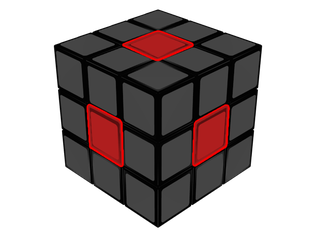
\includegraphics[width=0.30\textwidth]{figures/centers}
	}%
	\hfill
	\subcaptionbox{Aristas}{%
		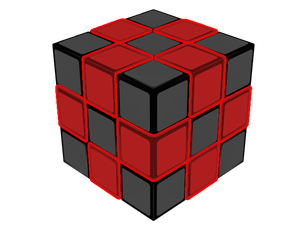
\includegraphics[width=0.30\textwidth]{figures/edges}
	}%
	\hfill
	\subcaptionbox{Esquinas}{%
		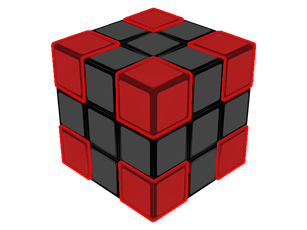
\includegraphics[width=0.30\textwidth]{figures/corners}
	}%
	\caption{Los 3 tipos de piezas del cubo de Rubik.}
\end{figure}

\subsection{Convenciones}
Existe una notación estándar para describir los ejes, las caras y los facelets del cubo.
Los 3 ejes de coordenadas del sistema de referencia utilizado se definen de la siguiente manera:
\begin{itemize}
	\item $x$: eje que atraviesa las caras derecha e izquierda del cubo, con respecto al observador.
	\item $y$: eje que atraviesa las caras superior e inferior del cubo.
	\item $z$: eje que atraviesa las caras frontal y trasera del cubo.
\end{itemize}
Así, cada una de las piezas esquina del cubo tiene 1 color por eje, mientras que las aristas tienen un color en sólo 2 ejes y los centros en solamente 1.

Las caras del cubo se identifican mediante la letra inicial de la palabra en inglés que identifica su posición con respecto al observador.
Éstas letras son \textit{U} (up), \textit{R} (right), \textit{F} (front), \textit{D} (down), \textit{L} (left) y \textit{B} (bottom).

\begin{figure}[h!]
	\centering
	\subcaptionbox{Ejes}{%
		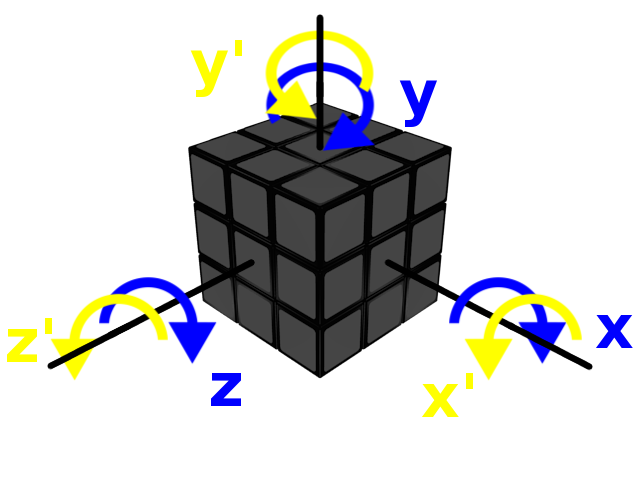
\includegraphics[width=0.45\textwidth]{figures/axes}
	}%
	\hfill
	\subcaptionbox{Caras}{%
		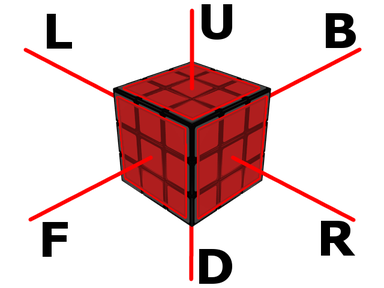
\includegraphics[width=0.45\textwidth]{figures/faces}
	}%
	\caption{Notación de ejes y caras del cubo.}
\end{figure}
De manera similar, los movimientos posibles de cada cara del cubo también quedan descritos por la letra correspondiente de la cara rotada.
En este punto, se decidió adoptar una notación ligeramente diferente de la estándar.
\textit{XN} indica que la cara \textit{X} rota en $90 \times N$ grados, donde los grados se miden utilizando la regla de la mano derecha sobre un vector normal a la superficie de la cara a rotar.
Entonces, por ejemplo \textit{R1} significa rotar la cara frontal en 90 (o -270) grados, \textit{R2} es rotar la cara frontal en 180 (o -180) grados y \textit{R3} rotar la cara frontal en 270 (o -90) grados.

\begin{figure}[h!]
	\centering
	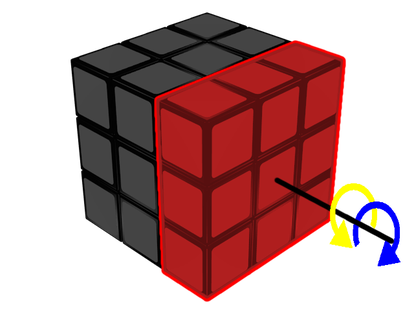
\includegraphics[scale=0.3]{figures/R1}
	\caption{Flecha azul: movimiento \textit{R1} ($90$ grados sentido horario). Flecha amarilla: movimiento \textit{R3} (90 grados sentido antihorario).}
	\label{moveR}
\end{figure}

Estos ángulos bastan para describir todos los movimientos posibles, ya que 360 equivale a una operación nula y cualquier otro ángulo dejaría el cubo en un estado inválido (bloqueando los movimientos de alguna de las demás caras).

Las piezas se identifican con las letras de las caras a las que pertenecen. Por lo tanto los centros son \textit{U}, \textit{R}, \textit{F}, \textit{D}, \textit{L} y \textit{B}, las aristas son \textit{UF}, \textit{UR}, \textit{UL}, \textit{UB}, \textit{DF}, \textit{DR}, \textit{DL}, \textit{DB}, \textit{FR}, \textit{FL}, \textit{BR} y \textit{BL} y las esquinas son \textit{URF}, \textit{URB}, \textit{ULF}, \textit{ULB}, \textit{DRF}, \textit{DRB}, \textit{DLF}, y \textit{DLB}.

El estado final del cubo se representó como un arreglo de 54 elementos, donde cada elemento representa un facelet. El orden de los facelets se muestra en la figura~\ref{faceletorder}.
La asignación de colores a cada cara es totalmente arbitraria y no tiene importancia para el sistema desarrollado. Lo importante es que una vez se decida una asignación se mantenga hasta el final.

\tikzset{boxu/.style={draw, minimum width=1cm, minimum height=1cm, fill=red, text=white}}
\tikzset{boxr/.style={draw, minimum width=1cm, minimum height=1cm, fill=blue, text=white}}
\tikzset{boxf/.style={draw, minimum width=1cm, minimum height=1cm, fill=yellow}}
\tikzset{boxd/.style={draw, minimum width=1cm, minimum height=1cm, fill=orange, text=white}}
\tikzset{boxl/.style={draw, minimum width=1cm, minimum height=1cm, fill=red, text=white}}
\tikzset{boxl/.style={draw, minimum width=1cm, minimum height=1cm, fill=green}}
\tikzset{boxb/.style={draw, minimum width=1cm, minimum height=1cm, fill=white}}
\tikzset{boxx/.style={draw, minimum width=1cm, minimum height=1cm, fill=red, text=white}}
\tikzset{boxy/.style={draw, minimum width=1cm, minimum height=1cm, fill=green}}
\tikzset{boxz/.style={draw, minimum width=1cm, minimum height=1cm, fill=blue, text=white}}
\tikzset{boxc/.style={draw, minimum width=1cm, minimum height=1cm}}

\begin{figure}[h!]
	\centering
	\begin{tikzpicture}[scale=0.8,every node/.style={scale=0.8}]
		\foreach \x in {0,...,2} {
			\foreach \y in {0,...,2} {
			 	\pgfmathsetmacro\result{int(3*\x+\y)}
				\node[boxu] at (3+\y, 8-\x) {$\result_U$};
			}
		}
		\foreach \x in {0,...,2} {
			\foreach \y in {0,...,2} {
				\pgfmathsetmacro\result{int(3*\x+\y + 36)}
				\node[boxl] at (\y, 5-\x) {$\result_L$};
			}
		}
		\foreach \x in {0,...,2} {
			\foreach \y in {0,...,2} {
				\pgfmathsetmacro\result{int(3*\x+\y + 18)}
				\node[boxf] at (\y+3, 5-\x) {$\result_F$};
			}
		}
		\foreach \x in {0,...,2} {
			\foreach \y in {0,...,2} {
				\pgfmathsetmacro\result{int(3*\x+\y + 9)}
				\node[boxr] at (\y+6, 5-\x) {$\result_R$};
			}
		}
		\foreach \x in {0,...,2} {
			\foreach \y in {0,...,2} {
				\pgfmathsetmacro\result{int(3*\x+\y + 45)}
				\node[boxb] at (\y+9, 5-\x) {$\result_B$};
			}
		}
		\foreach \x in {0,...,2} {
			\foreach \y in {0,...,2} {
				\pgfmathsetmacro\result{int(3*\x+\y + 27)}
				\node[boxd] at (\y+3, 2-\x) {$\result_D$};
			}
		}
	\end{tikzpicture}
	\caption{Orden de los facelets. El valor representa su posición el arreglo y el subíndice la cara a la que pertenece.}
	\label{faceletorder}
\end{figure}

\section{Sistema}
El sistema desarrollado consiste de varios módulos que pueden agruparse según su función en las siguientes categorías:
\begin{description}
	\item[Manipulación:] Módulos que se encargan de mover las articulaciones y grippers del robot.
	\item[Visión:] Módulos encargados de la detección del estado del cubo.
	\item[Resolución:] Modulo encargado de buscar una secuencia de rotaciones de caras que lleven al cubo a su estado resuelto.
\end{description}

\subsection{Manipulación}
Consiste de los módulos que se encargan de la parte hardware del sistema, es decir los movimientos de las articulaciones del robot y la apertura, cierre y calibración de los grippers. Para mover los brazos del robot se usa una combinación de cinemáticas inversas y manipulación directa de ángulos de sus articulaciones.

Las tareas requeridas incluyen:
\begin{enumerate}
	\item Recoger el cubo.
	\item Acercar el cubo a la cámara para detectar su estado.
	\item Realizar rotaciones de las caras.
	\item Mover el cubo de un brazo a otro cuando sea necesario.
\end{enumerate}

El robot Baxter posee varios tipos de grippers, mostrados en la figura~\ref{grippers}. Por el tamaño del cubo, se utilizó el gripper largo y angosto, para tener un agarre lo suficientemente profundo y apretado.

\begin{figure}[h!]
	\centering
	\includegraphics[width=0.25\textwidth]{figures/placeholder}
	\caption{Grippers disponibles.}
	\label{grippers}
\end{figure}

Los agarres son siempre de la forma como se muestra en la figura~\ref{agarres}. Esto impide la rotación de tres caras: las 2 que tocan los grippers y la cara que está más cercana al brazo del robot. La manera en que se realizan las rotaciones es que un brazo sostiene el cubo en una orientación cómoda para que el otro brazo se acerque y agarre una cara no bloqueada de manera perpendicular, y la gire en 90 180 o 270 grados según corresponda. Esto permite rotar libremente 3 caras. Para rotar las otras 3, se cambia el cubo al otro brazo, para que éste lo sostenga en una forma que libere las caras previamente bloqueadas.

\begin{figure}[h!]
	\centering
	\subcaptionbox{Agarre poco profundo, inestable.}{%
		\includegraphics[width=0.20\textwidth]{figures/placeholder}
	}%
	\hfill
	\subcaptionbox{Agarre utilizado. 3 caras libres para rotar. Estable}{%
		\includegraphics[width=0.20\textwidth]{figures/placeholder}
	}%
	\hfill
	\subcaptionbox{Agarre profundo, cara lejana bloqueada.}{%
		\includegraphics[width=0.20\textwidth]{figures/placeholder}
	}%
	\hfill
	\subcaptionbox{Agarre impreciso, cara lateral bloqueada. Inestable.}{%
		\includegraphics[width=0.20\textwidth]{figures/placeholder}
	}%
	\caption{Diferentes agarres.}
	\label{agarre}
\end{figure}

\subsubsection{Recogida}
La ejecución comienza con el cubo en la mesa, en una posición marcada cuyas coordenadas son conocidas. Los ejes se definieron con respecto al observador mirando de frente al robot, y no con respecto al punto de vista del robot. Utilizando el servicio de cinemáticas inversas de Baxter, se lleva el brazo izquierdo a una posición cercana al cubo, apuntando hacia abajo, para luego recogerlo, bloqueando las caras \textit{L}, \textit{R} y \textit{U}.

\begin{figure}[h!]
	\centering
	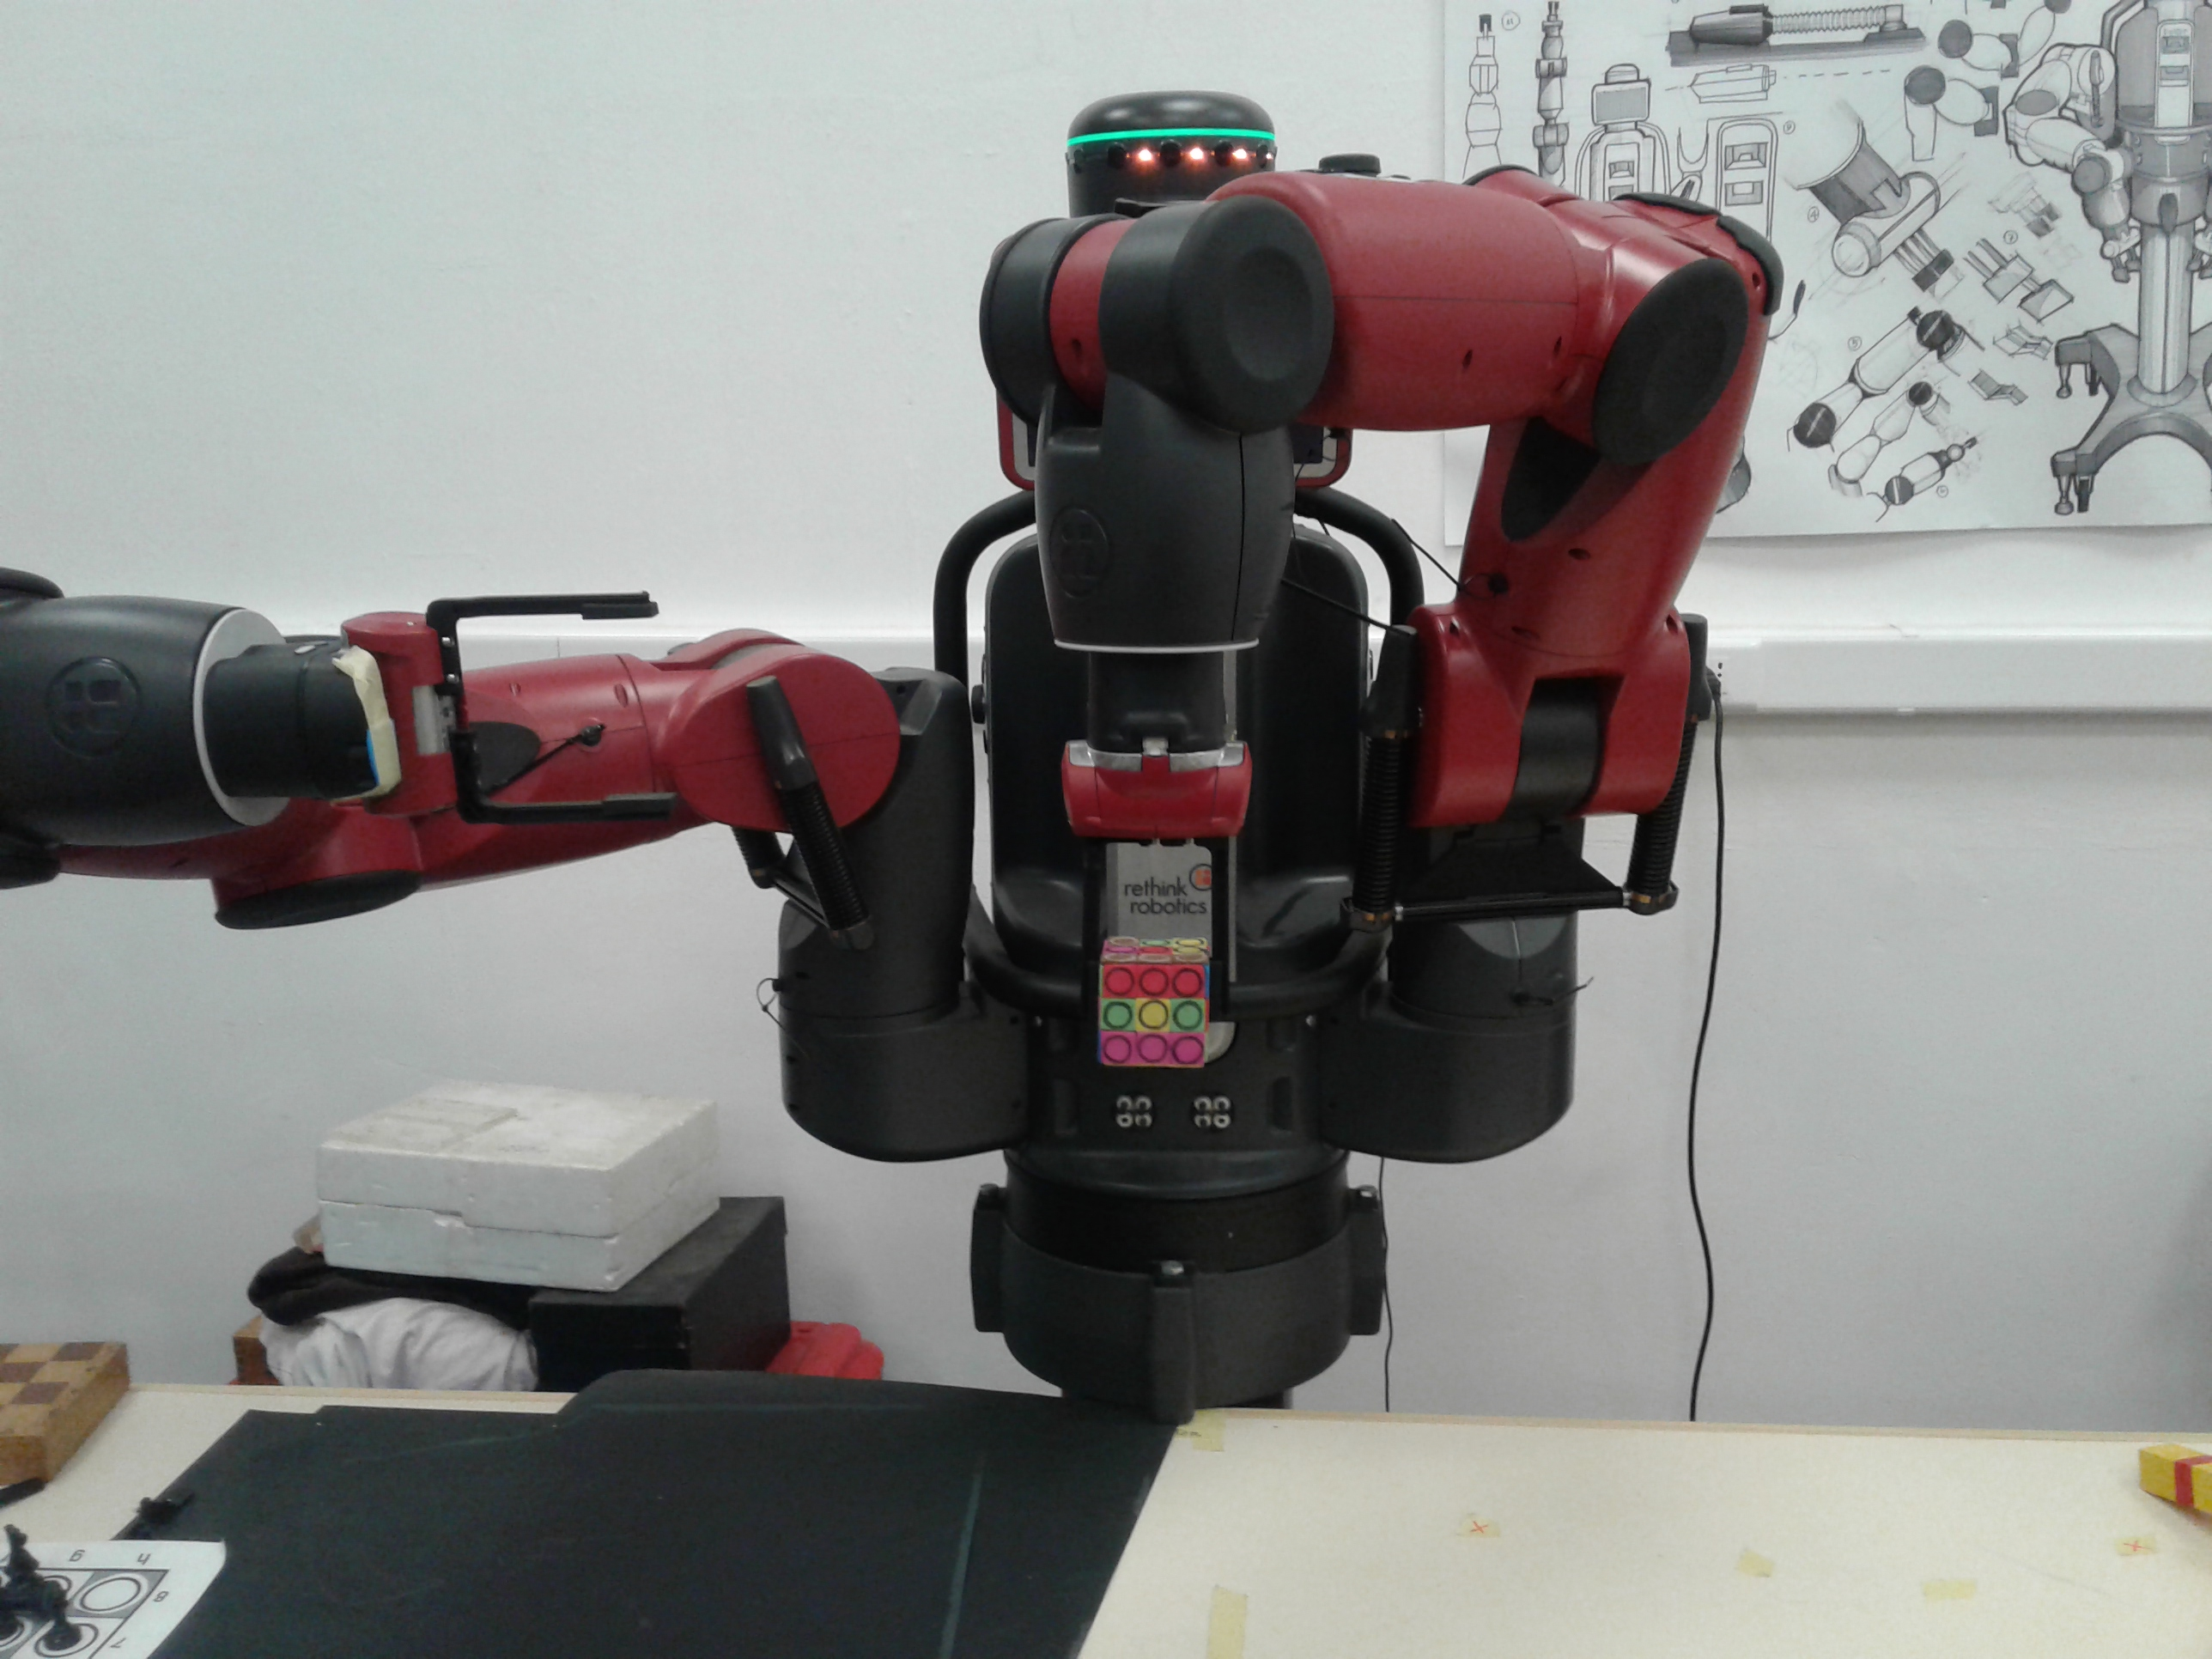
\includegraphics[scale=0.1]{figures/pick}
	\caption{Posición y orientación al recoger el cubo. Los grippers tocan las caras \textit{L} y \textit{R}.}
	\label{pick}
\end{figure}

\subsubsection{Acercamiento a cámara}
El servicio de cinemáticas inversas si bien garantiza la posición y orientación final solicitada para un gripper, no especifica nada sobre la trayectoria a realizar. Esto causa varios problemas, entre ellos los más graves son: la imposibilidad de llevar a cabo un movimiento debido a la complejidad de la trayectoria, a pesar de que sea una configuración válida; y la ejecución de ciertas trayectorias que causan que el robot se golpee a sí mismo. Debido a la naturaleza misma de IK, no es posible predecir cuándo suceden estos errores. Así que en este paso se mueve el brazo utilizando directamente los ángulos de cada una de sus articulaciones, para guiarlo a una configuración favorable, seguido inmediatamente por cinemáticas inversas para obtener la posición y orientación final deseada. Las 6 configuraciones necesarias para apuntar cada cara a la cámara se muestran en la figuras \ref{caml} y \ref{camr}.

\begin{figure}[h!]
	\centering
	\subcaptionbox{Capturando la cara \textit{F}}{%
		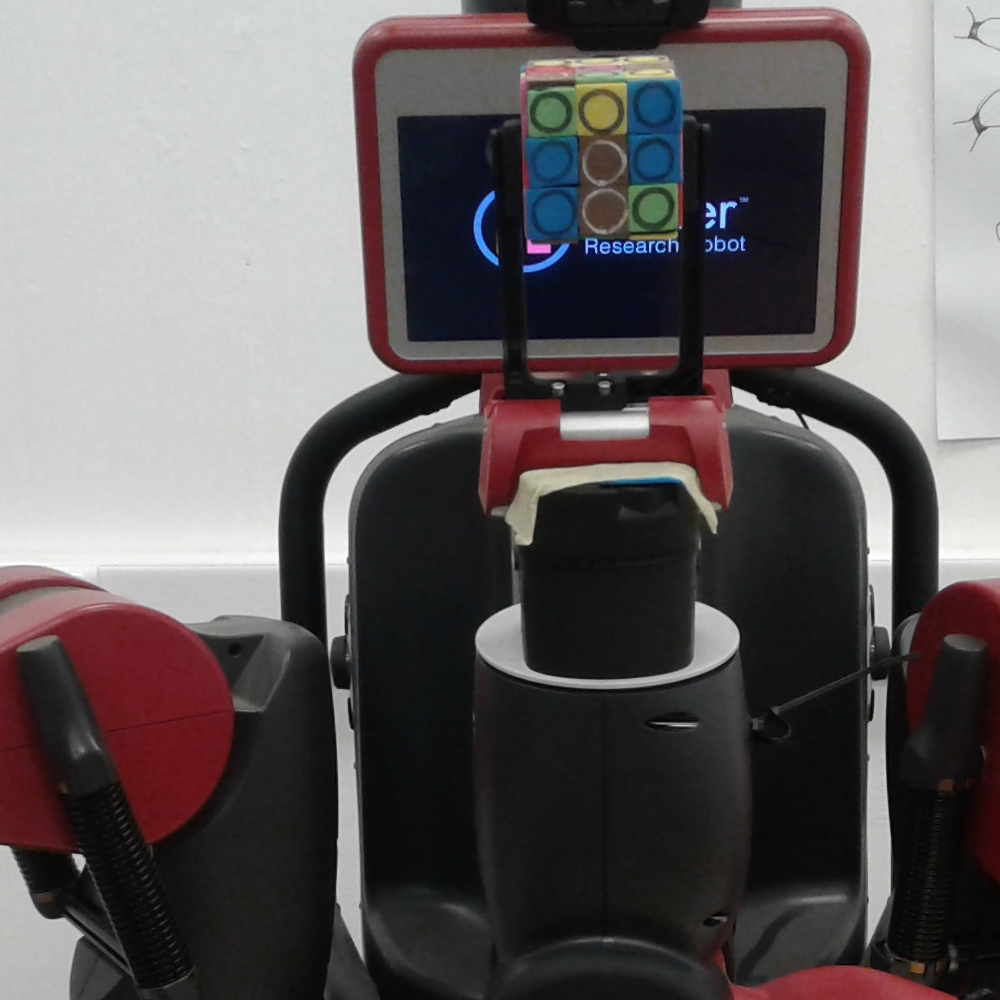
\includegraphics[width=0.30\textwidth]{figures/small_capture_F}
	}%
	\hfill
	\subcaptionbox{Capturando la cara \textit{D}}{%
		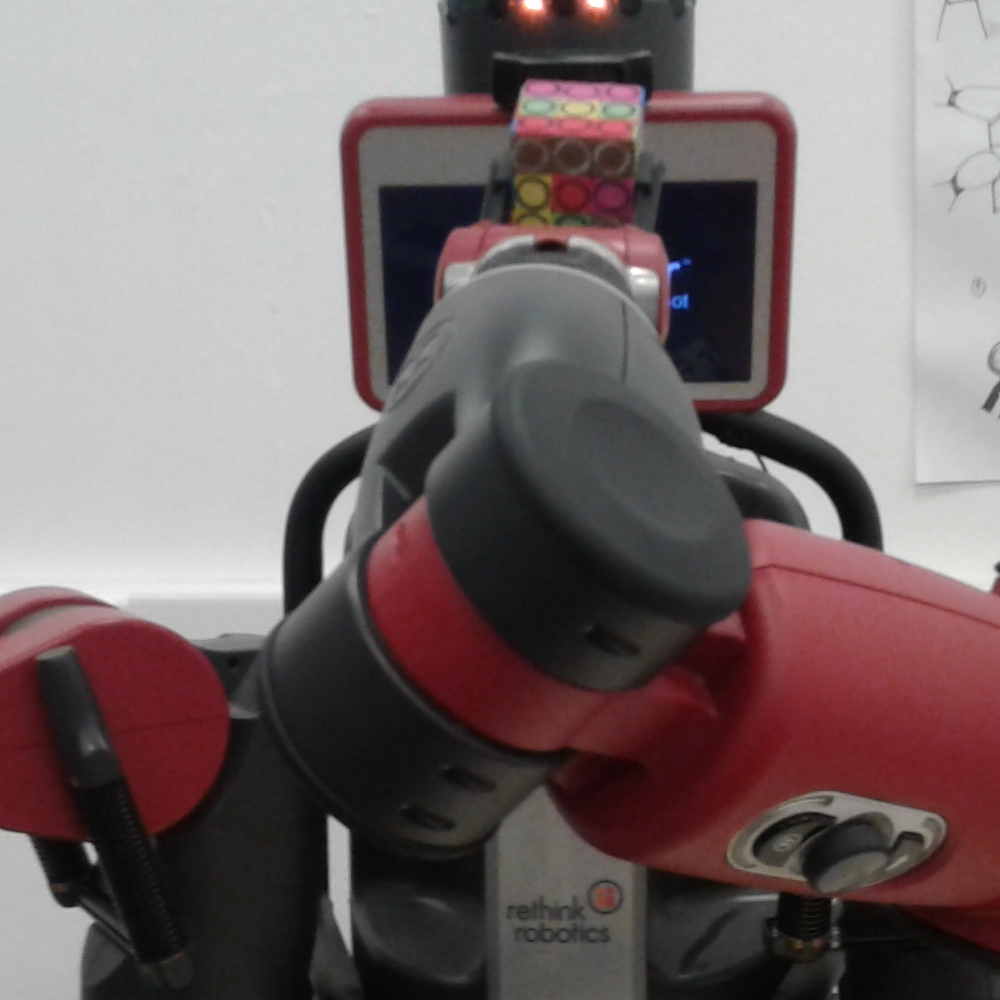
\includegraphics[width=0.30\textwidth]{figures/small_capture_D}
	}%
	\hfill
	\subcaptionbox{Capturando la cara \textit{B}}{%
		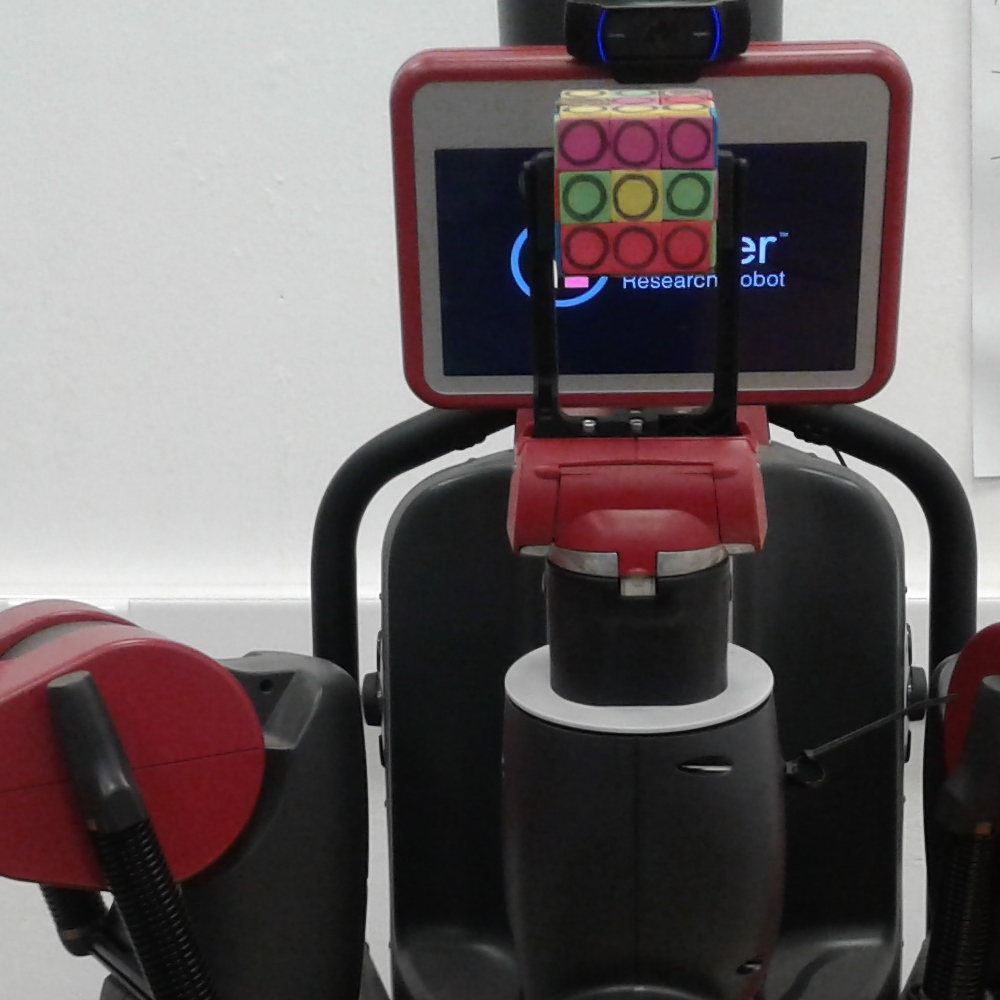
\includegraphics[width=0.30\textwidth]{figures/small_capture_B}
	}%
	\caption{Configuraciones del brazo izquierdo para acercamiento a la cámara.}
	\label{caml}
\end{figure}
\begin{figure}[h!]
	\centering
	\subcaptionbox{Capturando la cara \textit{L}}{%
		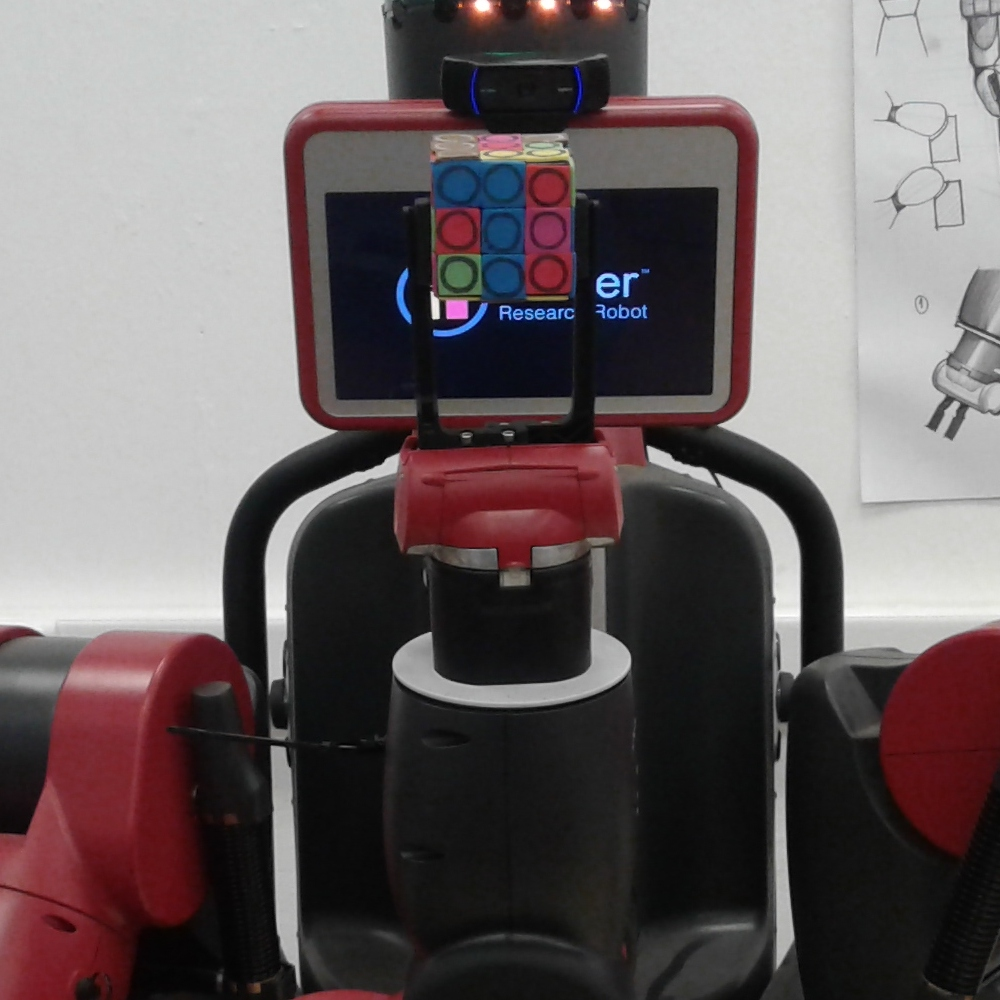
\includegraphics[width=0.30\textwidth]{figures/small_capture_L}
	}%
	\hfill
	\subcaptionbox{Capturando la cara \textit{U}}{%
		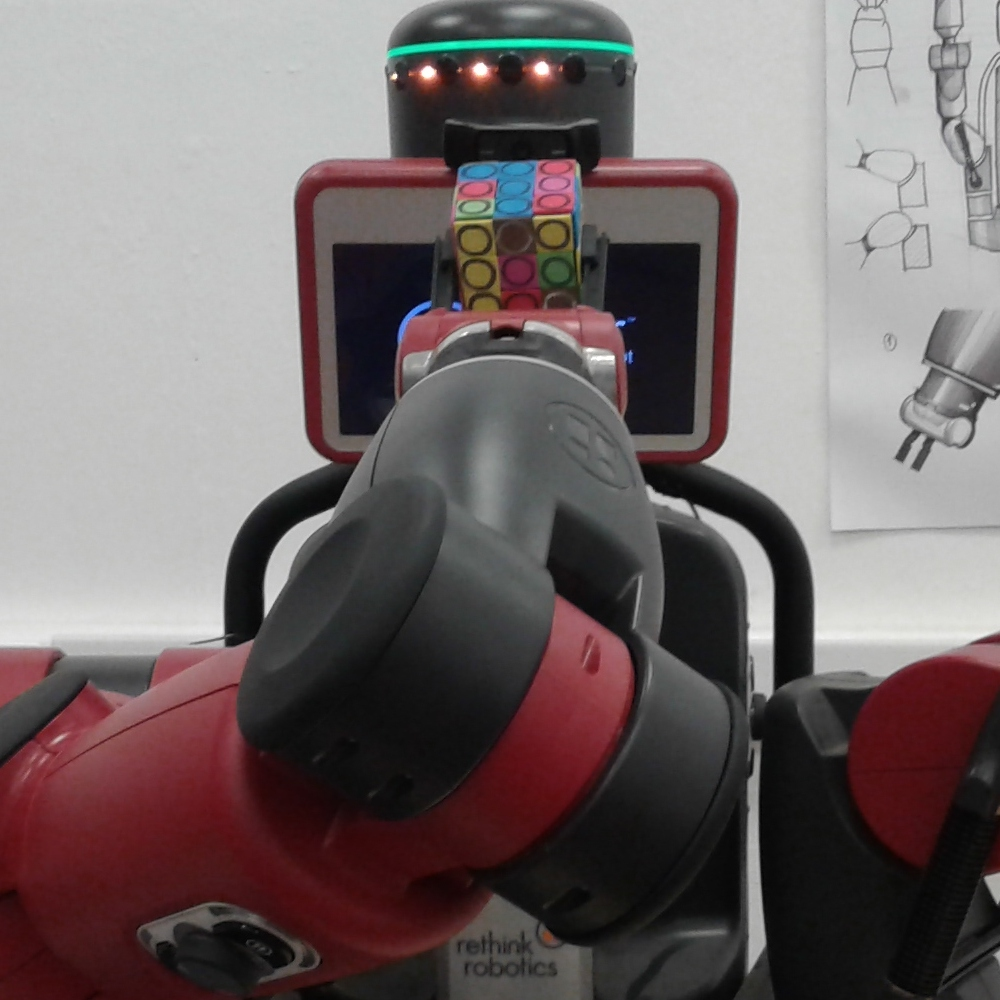
\includegraphics[width=0.30\textwidth]{figures/small_capture_U}
	}%
	\hfill
	\subcaptionbox{Capturando la cara \textit{R}}{%
		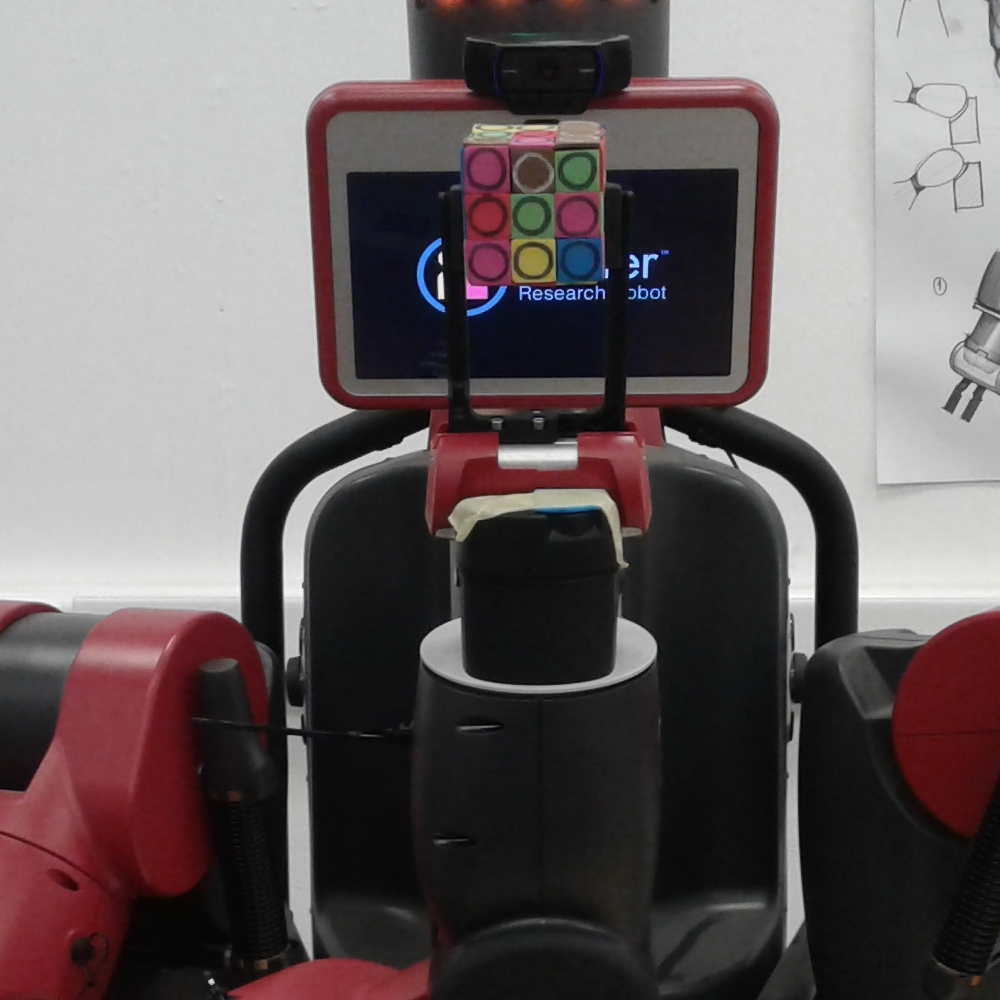
\includegraphics[width=0.30\textwidth]{figures/small_capture_R}
	}%
	\caption{Configuraciones del brazo derecho para acercamiento a la cámara.}
	\label{camr}
\end{figure}

\subsubsection{Rotaciones de caras}
Esta parte es muy similar a la anterior, en el sentido de que usa la misma idea de ángulos directos seguido por IK. Una diferencia es en las coordenadas utilizadas, para lo cual se escogió una posición en la que el robot pudiese llegar en las 3 orientaciones de cada brazo. Estas configuraciones se muestran en las figuras \ref{movel} y \ref{mover}.

\begin{figure}[h!]
	\centering
	\subcaptionbox{Rotación cara \textit{F}}{%
		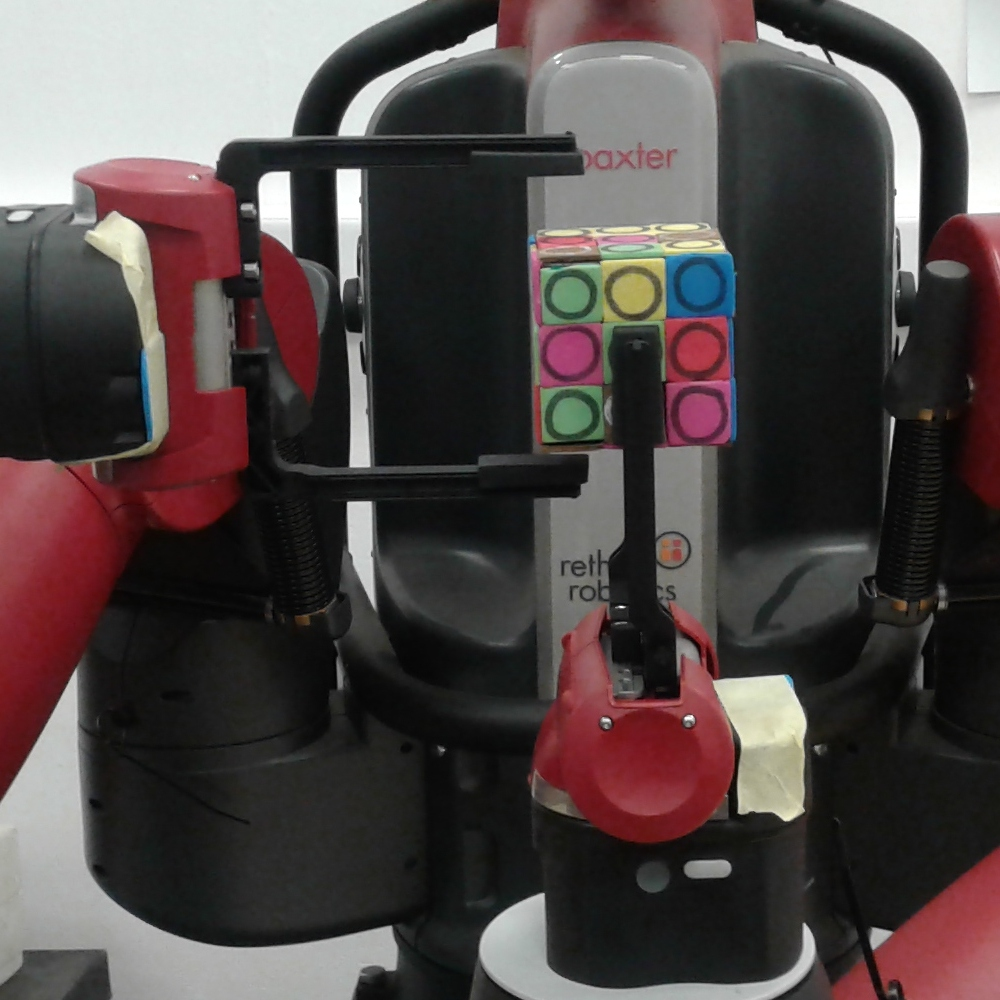
\includegraphics[width=0.30\textwidth]{figures/small_move_F}
	}%
	\hfill
	\subcaptionbox{Rotación cara \textit{D}}{%
		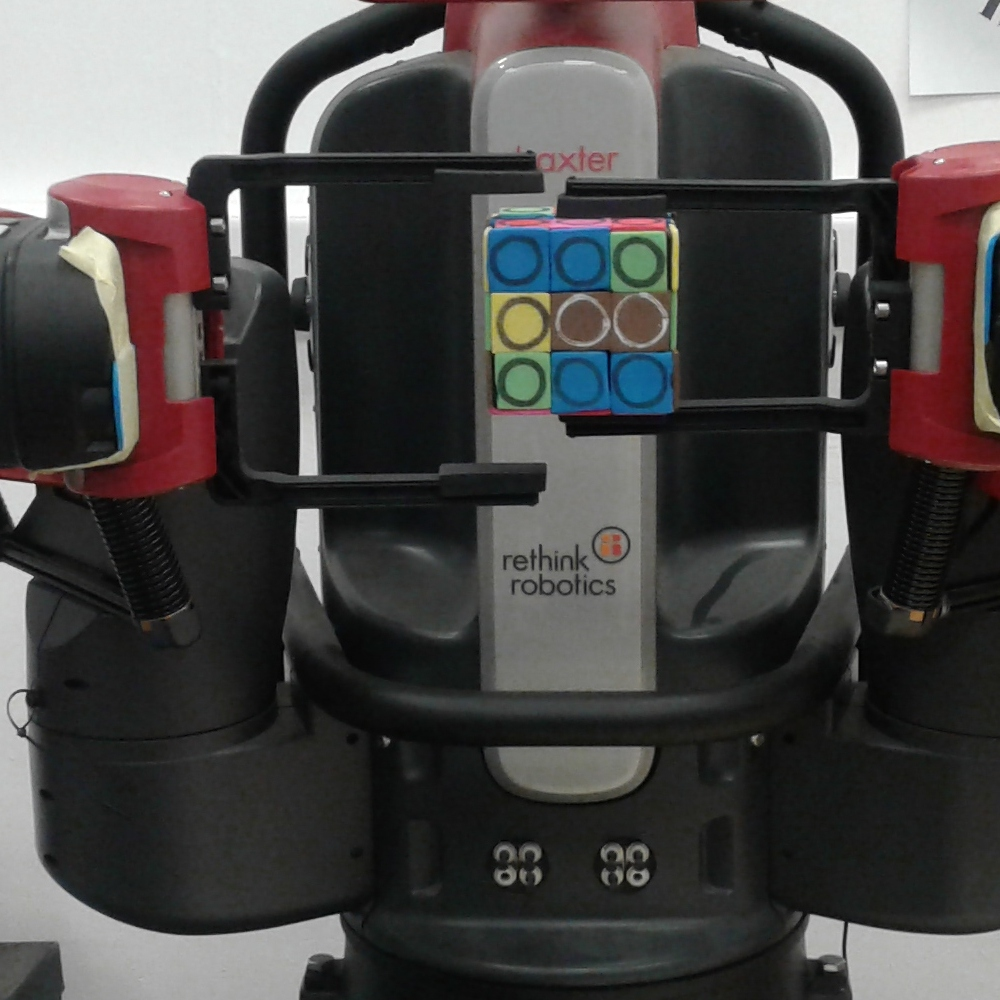
\includegraphics[width=0.30\textwidth]{figures/small_move_D}
	}%
	\hfill
	\subcaptionbox{Rotación cara \textit{B}}{%
		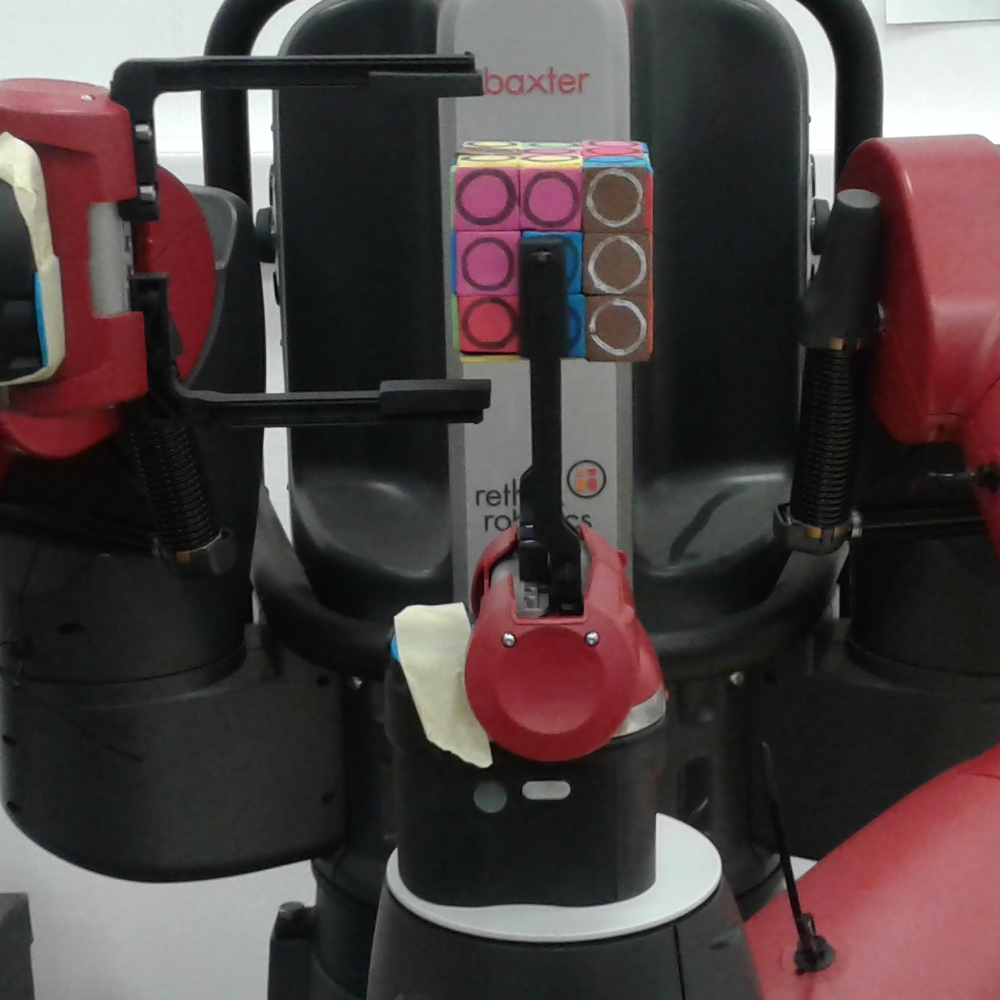
\includegraphics[width=0.30\textwidth]{figures/small_move_B}
	}%
	\caption{Configuraciones del brazo izquierdo para rotaciones.}
	\label{movel}
\end{figure}
\begin{figure}[h!]
	\centering
	\subcaptionbox{Rotación cara \textit{L}}{%
		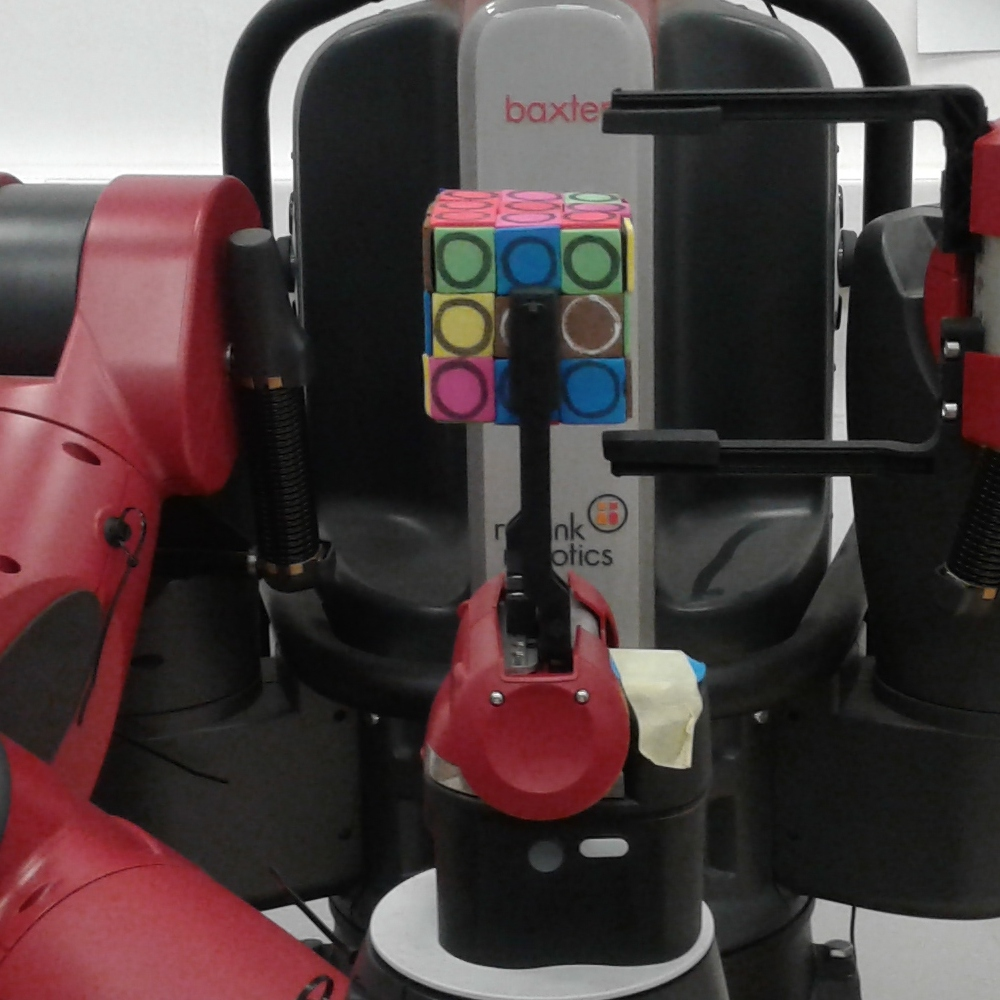
\includegraphics[width=0.30\textwidth]{figures/small_move_L}
	}%
	\hfill
	\subcaptionbox{Rotación cara \textit{U}}{%
		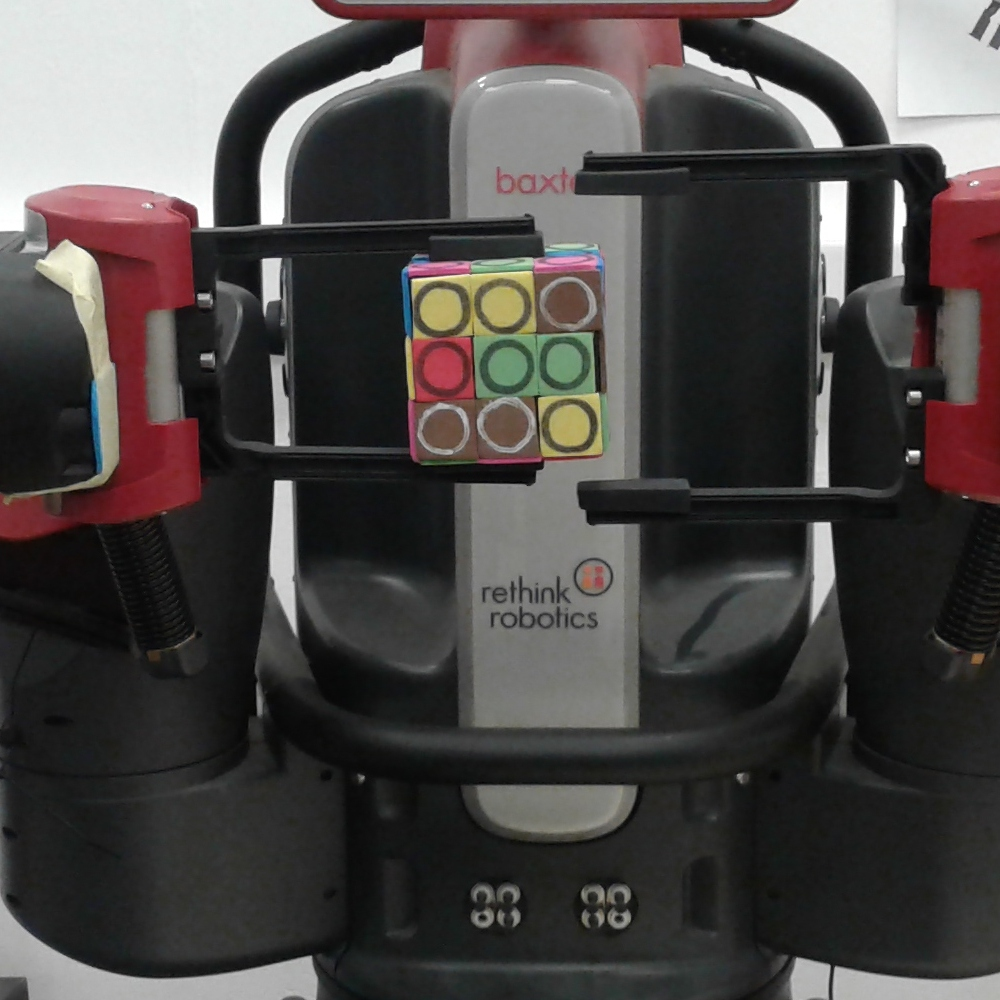
\includegraphics[width=0.30\textwidth]{figures/small_move_U}
	}%
	\hfill
	\subcaptionbox{Rotación cara \textit{R}}{%
		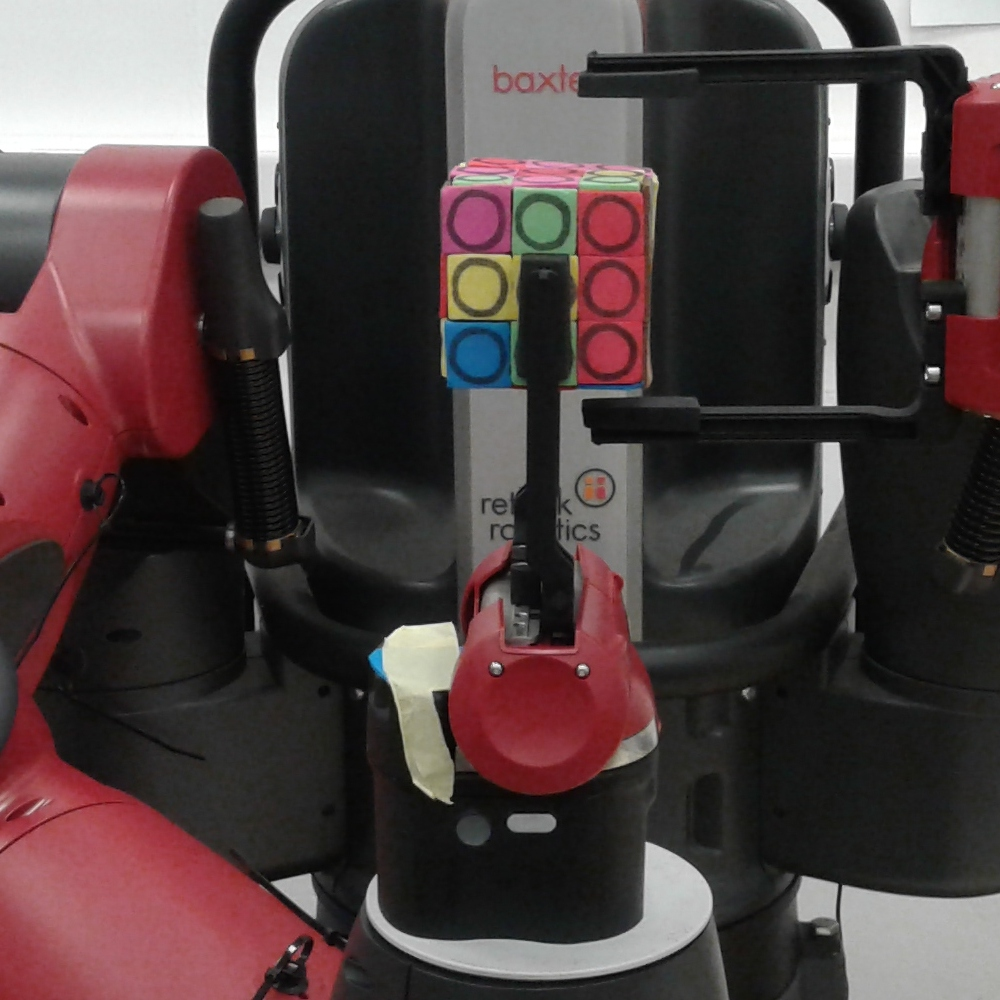
\includegraphics[width=0.30\textwidth]{figures/small_move_R}
	}%
	\caption{Configuraciones del brazo derecho para rotaciones.}
	\label{mover}
\end{figure}
Otra diferencia es que en este paso se agregan posiciones intermedias al acercar el brazo libre a la posición del cubo, para que el servicio de cinemáticas inversas prefiera movimientos paralelos y no cause golpes no deseados. Ver figura ....

Para efectuar una rotación de alguna cara, la secuencia de pasos es:
\begin{enumerate}
	\item Brazo que sostiene el cubo se mueve a una posición definida en función de la cara que será rotada (ángulos directos).
	\item Brazo libre se mueve a una posición cercana a la cara a rotar del cubo, pero no lo suficiente para agarralo (IK).
	\item Brazo libre se mueve a una posición aún mas cercana a la cara a rotar del cubo, lo suficiente para agarralo (IK, movimiento paralelo).
	\item Gripper de brazo libre se cierra.
	\item brazo libre rota articulación de su muñeca en el ángulo deseado (águlos directos).
	\item Gripper de brazo libre se abre.
	\item brazo libre se aleja del brazo que sostiene el cubo para permitir libertad en los movimientos siguientes (IK, seguido de angulos directos).
\end{enumerate}

\subsubsection{Cambio de mano}
Este paso utiliza ángulos directos y cinemáticas inversas. Las posiciones para realizar este paso son las mismas de los brazos ocupados para los movimientos \textit{U} y \textit{R} respectivamente, con la diferencia de que el brazo izquierdo tiene un desplazamiento de 90 grados. Así, cuando se cambia el brazo de la mano izquierda a la derecha, se liberan las caras \textit{L}, \textit{R} y \textit{U}, pero se bloquean las caras \textit{F}, \textit{B} y \textit{L}, y viceversa.

\begin{figure}[h!]
	\centering
	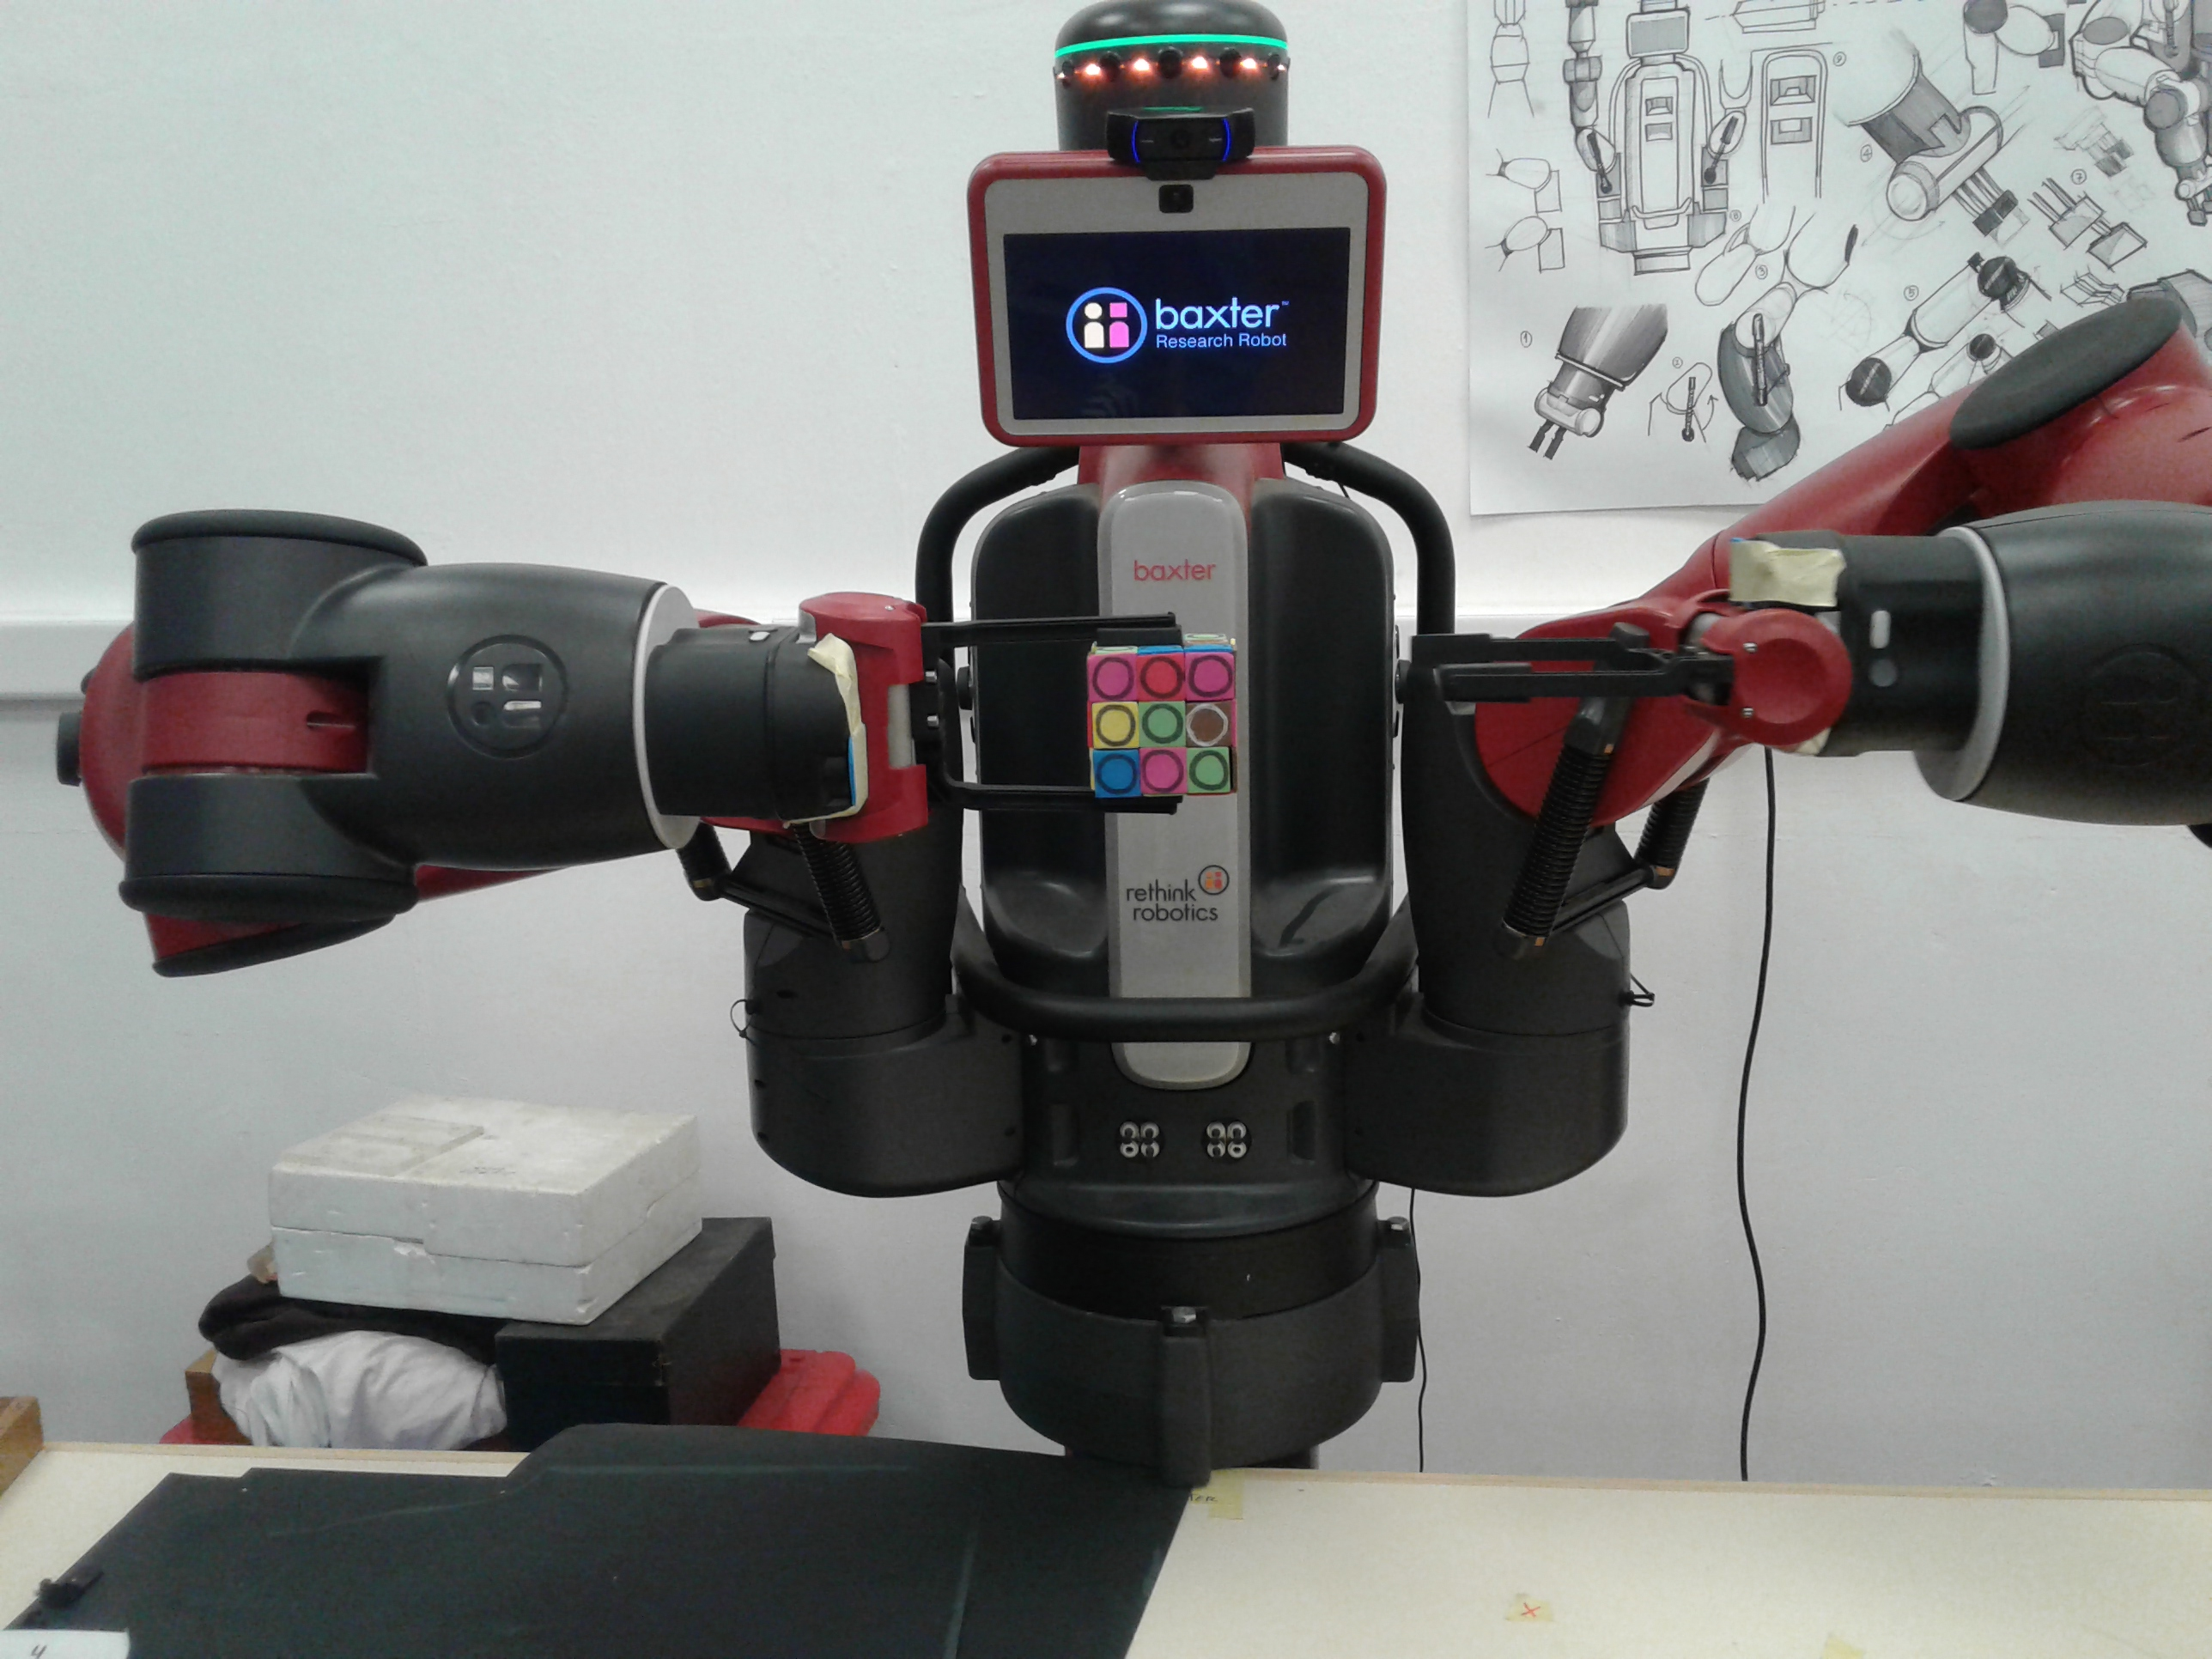
\includegraphics[scale=0.1]{figures/switch}
	\caption{Cambio de mano}
	\label{switch}
\end{figure}

Al tener 3 caras libres por brazo, puede que se necesiten pocos cambios de mano para realizar una secuencia de giros. Sin embargo, en el peor caso siempre se tendrá tantos cambios de mano como rotaciones se vaya a realizar.

\subsection{Visión}
Estos módulos se encargan de obtener el estado del cubo. Es la parte más compleja del sistema.
\subsubsection{Preparaciones previas}
\subsubsection{Robot}
Si bien Baxter posee cámaras en sus 2 manos y en su cabeza, la calidad de la imagen que obtiene usándolas deja bastante que desear. Se decidió entonces utilizar una cámara externa, la cual se ubicó encima de la cámara de la cabeza del robot. Ésta fue conectada directamente a la máquina desde donde se ejecuta el programa principal, pues a pesar de que el robot tiene interfaces USB (que permite el uso de joysticks entre otras cosas) no se encontró documentación ni códigos de ejemplo respecto del uso de cámaras externas.
\begin{figure}[h!]
	\centering
	\subcaptionbox{Cámara brazo izquierdo.}{%
		\includegraphics[width=0.20\textwidth]{figures/placeholder}
	}%
	\hfill
	\subcaptionbox{Cámara brazo derecho.}{%
		\includegraphics[width=0.20\textwidth]{figures/placeholder}
	}%
	\hfill
	\subcaptionbox{Cámara de la cabeza.}{%
		\includegraphics[width=0.20\textwidth]{figures/placeholder}
	}%
	\hfill
	\subcaptionbox{Cámara externa.}{%
	\includegraphics[width=0.20\textwidth]{figures/placeholder}
	}%
	\caption{Calidad de imagen de las distintas cámaras disponibles.}
	\label{camaras}
\end{figure}

\subsubsection{Cubo}
El cubo fue cubierto con goma eva. Esto cumple varios objetivos. En primer lugar, es un material que refleja la luz más difusamente que el plástico de los stickers del cubo, por lo que los colores capturados por la cámara tienden a ser más uniformes, como se aprecia en la figura~\ref{luz}.

\begin{figure}[h!]
	\centering
	\subcaptionbox{Luz sobre el plástico. Algunos colores son erróneamente detectados como blanco.}{%
	\includegraphics[width=0.40\textwidth]{figures/placeholder}
	}%
	\subcaptionbox{Luz sobre la goma eva. }{%
	\includegraphics[width=0.40\textwidth]{figures/placeholder}
	}%
	\caption{Difusión de luz en ambos materiales.}
	\label{luz}
\end{figure}

En segundo lugar, la goma eva aumenta el roce entre los grippers y el cubo, ya que el plástico original tendía a deslizarse con mayor facilidad. Por último pero no menos importante, provee algo de protección cuando el cubo cae al suelo, algo que sucedió no pocas veces.

Sobre cada facelet del cubo de dibujó un círculo para marcar las regiones de interés. Esto ayuda mucho a la detección.

Los colores de goma eva utilizados fueron rojo, azul, verde, amarillo, rosado y marrón, correspondientes a los mismo colores originales con excepción de los 2 últimos (naranja y blanco, originalmente).

\begin{figure}[h!]
	\centering
	\subcaptionbox{Cubo original, caras \textit{U} \textit{R} y \textit{F}.}{%
	\includegraphics[width=0.20\textwidth]{figures/placeholder}
	}%
	\subcaptionbox{Cubo original, caras \textit{D} \textit{L} y \textit{B}.}{%
	\includegraphics[width=0.20\textwidth]{figures/placeholder}
	}%
	\subcaptionbox{Cubo cubierto, caras \textit{U} \textit{R} y \textit{F}.}{%
	\includegraphics[width=0.20\textwidth]{figures/placeholder}
	}%
	\subcaptionbox{Cubo cubierto, caras \textit{D} \textit{L} y \textit{B}.}{%
	\includegraphics[width=0.20\textwidth]{figures/placeholder}
	}%
	\caption{Colores.}
	\label{colorescubo}
\end{figure}

\subsubsection{Círculos de Hough}
Una vez que el manipulador acerca el cubo a la cámara, se capturan fotos de cada cara. Sobre cada una de estas 6 imágenes, se aplica el algoritmo de Hough para detección de círculos, provisto por la biblioteca de OpenCV. El algoritmo itera hasta que encuentra exactamente 9 círculos en cada imagen, entregando sus centros y radios respectivos.

\begin{figure}[h!]
	\centering
	\subcaptionbox{Detección correcta.}{%
		\includegraphics[width=0.30\textwidth]{figures/placeholder}
	}%
	\subcaptionbox{Detección incorrecta, faltan círculos.}{%
		\includegraphics[width=0.30\textwidth]{figures/placeholder}
	}%
	\subcaptionbox{Detección incorrecta, sobran círculos.}{%
		\includegraphics[width=0.30\textwidth]{figures/placeholder}
	}%
	\caption{Identificación de círculos.}
	\label{circulos}
\end{figure}
Este algoritmo funciona asi... TODO
Los parámetros usados se obtuvieron mediante ensayo y error, y corresponden a TODO.

\subsubsection{Colores representantes}
Una vez se tienen los 54 círculos, se procede a extraer un color representativo de la región encerrada por cada uno. Se decidió usar la mediana RGB, pues en el caso de una detección imperfecta de un círculo no se quiere que el borde del círculo afecte al color representante. Para mayor comodidad en la iteración, se utilizó como región un cuadrado inscrito en un círculo en lugar del círculo completo. Este paso tiene como resultado un vector 54 colores RGB.

\subsubsection{Clasificación}
Para identificar cuales facelets son del mismo color, independientemente de cual sea éste, se utilizó un modelo no supervisado para clasificarlos. El algoritmo utilizado fue el de mezcla de gaussianas (Gaussian Mixture Model, o \textit{GMM}), con 6 componentes. Las características usadas fueron las componentes matiz y saturación de la conversión a HSV de cada uno de los colores RGB representantes de cada facelet.

\begin{figure}[h!]
	\centering
	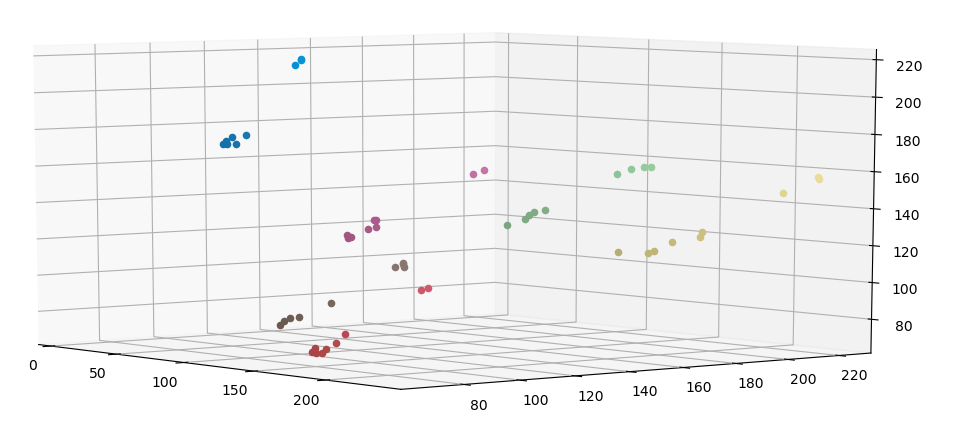
\includegraphics[width=0.8\textwidth]{figures/rgb_3d}
	\caption{Colores representantes en espacio RGB.}
	\label{rgb3d}
\end{figure}


Empíricamente se observó que la distribución RGB de los colores son de la misma cara se alinean en rectas. Después de fracasar con varios modelos (KMeans, KMeans despúes de PCA, KMeans en HSV) se decidió optar por un modelo de mezcla de gaussianas en HSV, pues los colores, con excepción del marrón tienen componentes de matiz muy similares, variando principalmente en su saturación o brillo.

\begin{figure}[h!]
	\centering
	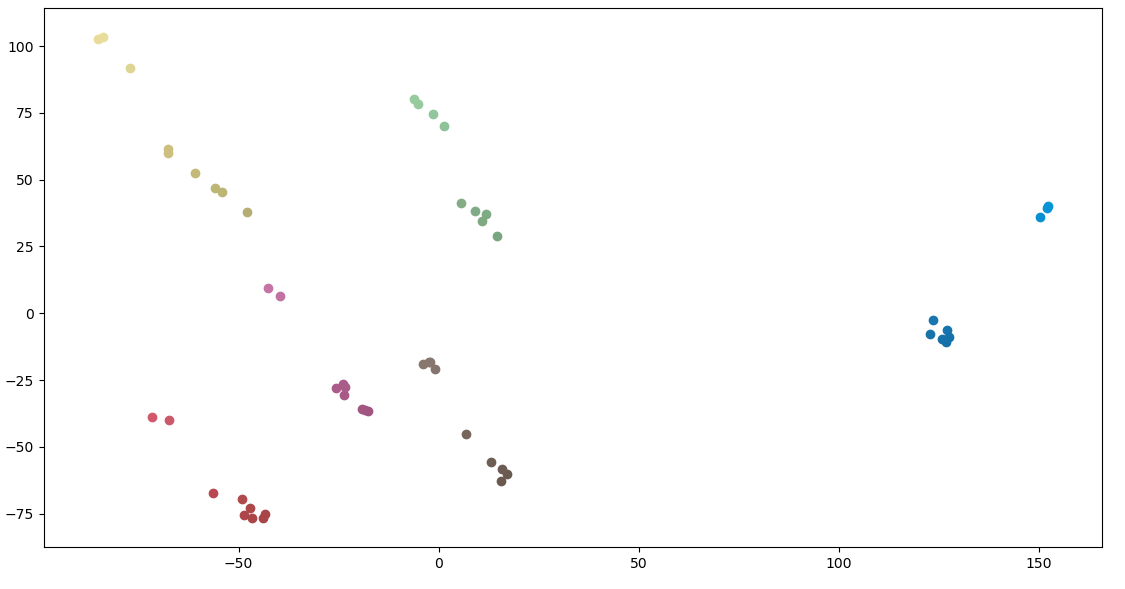
\includegraphics[width=0.8\textwidth]{figures/rgb_pca}
	\caption{Colores representantes, luego de aplicar PCA con 2 componentes. Clases no trivialmente separables.}
	\label{rgb3d}
\end{figure}

Aprovechando el hecho de que las piezas centro del cubo no se mueven, se puede saber con certeza de que esos colores son todos distintos, no así las aristas y esquinas del cubo que pueden moverse libremente a cualquier otra ubicación. Los colores de los centros se utilizaron entonces como las medias iniciales de las gaussianas. Además, se asignaron las probabilidades a priori en 1/6 a cada gaussiana, pues todas las caras tienen la misma cantidad de facelets. Las covarianzas iniciales de cada gaussiana se tomaron con mayor varianza en el eje de saturación que en el de matiz. Esto es simplemente conocimiento previo de la distribución de los datos luego de un montón de intentos.

\begin{figure}[h!]
	\centering
	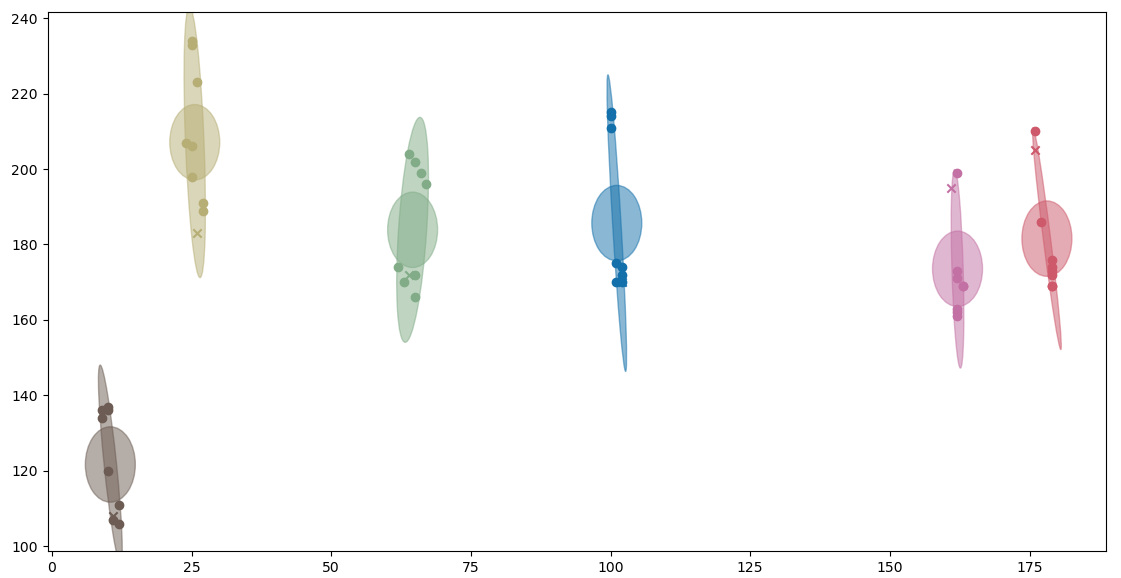
\includegraphics[width=\textwidth]{figures/gmm}
	\caption{Colores representantes, en HSV. Eje horizontal es matiz, eje vertical es saturación. Los puntos marcados con cruces indican los representantes de los centros, y por ende las medias iniciales de las gaussianas. Las elipses grandes son las covarianzas finales, a 2 desviaciones estándar las elipses pequeñnas son las covarianzas iniciales. Esta clasificación es correcta.}
	\label{gmmgood}
\end{figure}

\begin{figure}[h!]
	\centering
	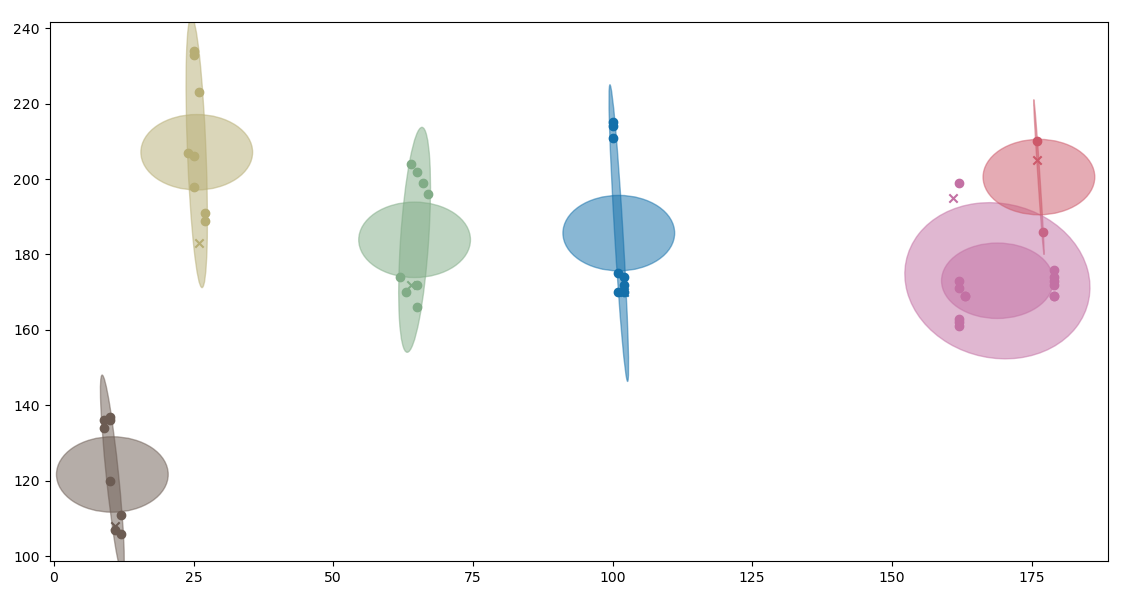
\includegraphics[width=\textwidth]{figures/gmm_bad}
	\caption{El mismo caso de la figura~\ref{gmmgood}. Cuando las covarianzas crecen por igual en ambos ejes, ocurren más errores de clasificación, al igual que con KMeans. En particular, puntos rojos fueron incorrectamente clasificados como puntos rosados.}
	\label{gmmbad}
\end{figure}

Cuando GMM era incializado con KMeans, como lo hace por ejemplo el modelo GMM de la biblioteca de Python scikit-learn, se tiende a confundir los colores rojo y rosado, ya que sus matices suelen están más cerca que la distancia en saturación más grande entre 2 rojos o 2 rosados.

Al finalizar este paso, si es que no hubo algún error de clasificación, se tiene un vector de 54 caracteres en el orden dado por la figura\ref{faceletorder}. Así, el caracter \textit{X} en la posición $i$ indica que el facelet $i$ es del mismo color que el centro de la cara \textit{X}. Por ejemplo, para los representantes de las figuras ..., el estado resultante es el string \textit{LLLFUBRUBRRFRRUDBBFFUDFUDRRLFFBDDBRRBLUDLFDLFUUUBBLDDL}.


\subsection{Resolución}
Para la fase de resolución se utilizó el algoritmo de 2 fases de Kociemba. Se adaptó la implementación de [referencia] a las necesidades del sistema desarrollado, además de portarlo al lenguaje Python 2 para integrarlo facilmente a los demás módulos.

Este módulo recibe un string con el estado o permutación del cubo y entrega una secuencia de giros en el formato descrito en la sección [referencia]. Por ejemplo, para el mismo string mostrado en la sección anterior (\textit{LLLFUBRUBRRFRRUDBBFFUDFUDRRLFFBDDBRRBLUDLFDLFUUUBBLDDL}), la secuencia de giros que lleva al cubo a su estado resuelto es \textit{B1 L1 D1 R1}. Obsérvese que para que el robot realice dicha secuencia de acciones, si comienza con el cubo en su brazo izquierdo podrá realizar la rotación \textit{B1} inmediatamente. Sin embargo, como el gripper izquierdo bloquea las caras \textit{L} y \textit{R} y \textit{U}, se deberá realizar un cambio de mano antes de realizar el giro \textit{L1}. Lo mismo sucederá cuando posteriormente se quiera efectuar \textit{D1} con el cubo en el brazo derecho y \textit{R1} con el cubo en el brazo izquierdo.


\subsection{Orden de ejecución final}
El orden de ejecución final es el siguiente:
\begin{enumerate}
	\item Robot recoge el cubo de Rubik con su brazo izquierdo. La posición donde queden ubicados los grippers corresponderán a las caras \textit{R} y \textit{L}.
	\item Robot mueve brazo izquierdo de manera de apuntar las caras \textit{F}, \textit{B} y \textit{D} (en ese orden) directamente hacia la cámara ubicada en su cabeza. Cada cara es fotografiada una vez y se guarda la matriz correspondiente a la imagen RGB y los 9 círculos detectados en cada cara.
	\item Robot entrega el cubo de su mano izquierda a su mano derecha.
	\item Robot mueve brazo derecho de manera de apuntar las caras \textit{R}, \textit{L} y \textit{U} (en ese orden) directamente hacia la cámara ubicada en su cabeza. Cada cara es fotografiada una vez y se guarda la matriz correspondiente a la imagen RGB y los 9 círculos detectados en cada cara.
	\item Se extrae el color representativo de cada uno de los 54 círculos, dando a lugar a un arreglo de 54 colores RGB.
	\item Se agrupan los colores del paso anterior para obtener el estado del cubo, como una permutación.
	\item Se toma la permutación obtenida y se obtiene una secuencia de rotaciones para resolver el cubo.
	\item Se realizan las rotaciones moviendo los brazos del robot, cambiando de mano cuando sea necesario.
\end{enumerate}

\chapter{Experimentos y resultados}

Se realizaron 2 tipos de experimentos, de visión y de manipulación. Pruebas de resolución no se llevaron a cabo, ya que el solucionador siempre encuentra una solución, a menos que el cubo se encuentre en un estado inválido.

Se utilizó el scrambler legacy de la World Cube Association, para generar 20 permutaciones del cubo de Rubik. Cada una de estas permutaciones, también llamados ``desarmes'' consiste de 30 rotaciones, y fueron aplicadas manualmente sobre el cubo. La tabla \ref{vision} del apéndice muestra las secuencias de rotaciones utilizadas en cada experimento.

\section{Visión}
Para la visión, se utilizaron los 20 desarmes en su totalidad. Cada ejecución comenzó con el robot recogiendo el cubo desde una mesa.

\begin{figure}[h!]
	\centering
	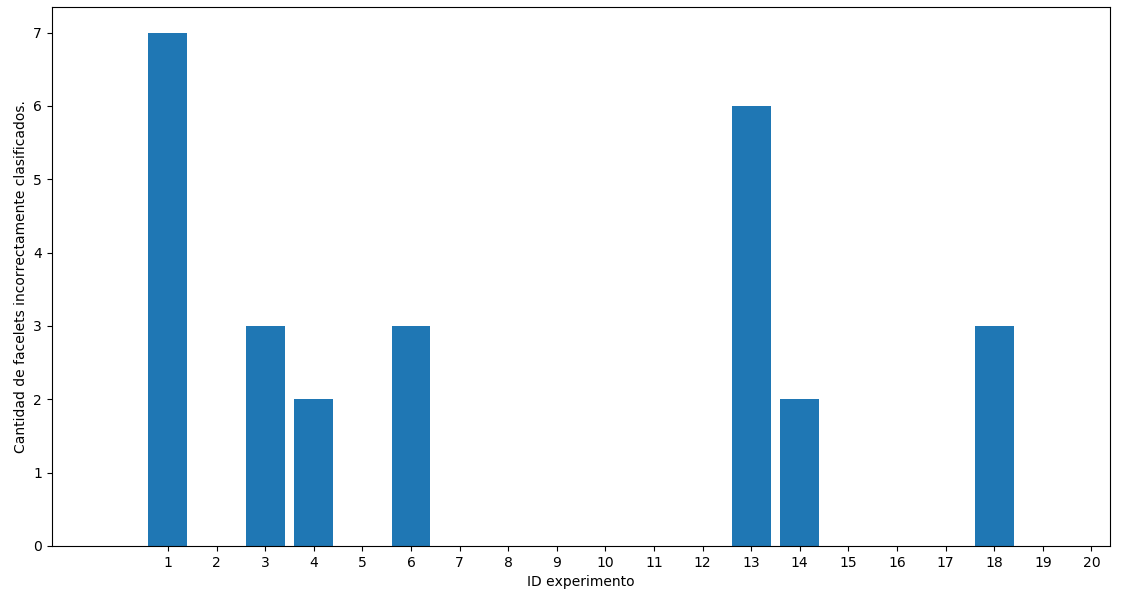
\includegraphics[width=\textwidth]{figures/error_facelet}
	\caption{Facelets mal clasificados por cada prueba realizada.}
	\label{erroresfacelets}
\end{figure}
Del total de pruebas, el 65\% no tuvo errores de clasificación. La cantidad de facelets mal clasificados en promedio fue de 1.3 facelets, con desviación estándar de 2.076. La cantidad de facelets mal clasificados en cada experimento se muestra en la figura\ref{erroresfacelets}. En la tabla\ref{visionerrors} del apéndice, se muestra específicamente cuales fueron los estados del cubo en cada ejecución, y exactamente cúales fueron los faceles indebidamente clasificados.

Respecto a la totalidad de facelets en todos los experimentos, el 97.6\% fue etiquetado correctamente. Lamentablemente, basta con 1 sólo facelet incorrecto para que el solver sea incapaz de encontrar una solución, por lo que en el mejor de los casos el robot hubiese sido capaz de resolver el 65\% de estos desarmes.

\begin{figure}[h!]
	\centering
	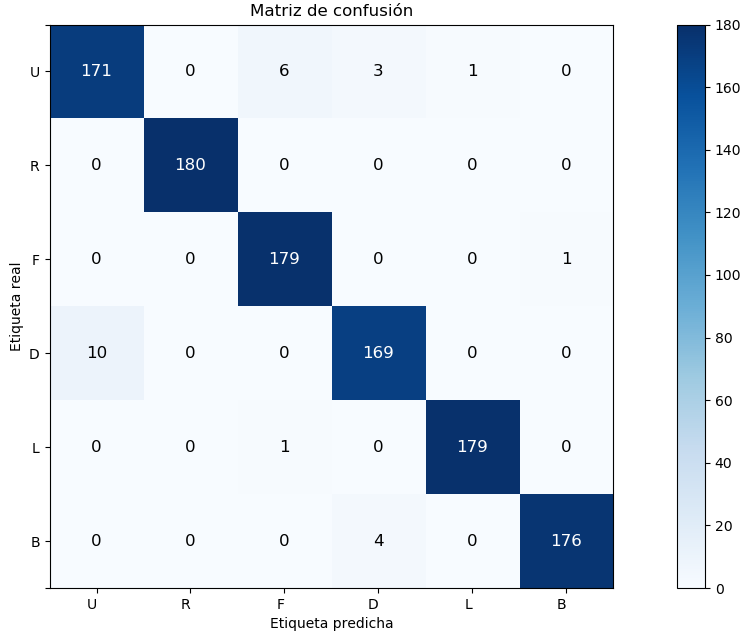
\includegraphics[width=0.7\textwidth]{figures/conf_matrix}
	\caption{Matriz de confusión de predicción de colores, sin normalizar.}
	\label{confusion}
\end{figure}
\begin{figure}[h!]
	\centering
	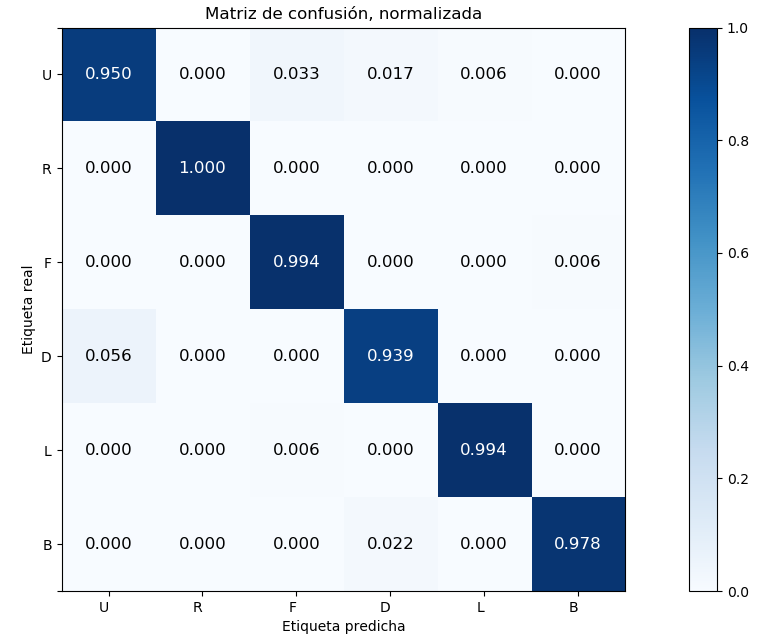
\includegraphics[width=0.7\textwidth]{figures/conf_matrix_norm}
	\caption{Matriz de confusión de predicción de colores, normalizada.}
	\label{confusionnorm}
\end{figure}

Una parte importante de los errores se dieron entre las caras U y D, que en las pruebas realizadas correspondieron a los colores rojo y rosado. Estos colores son muy similares entre sí, aunque esto depende mucho de las condiciones de iluminación del ambiente donde se encuentre el robot. El detalle de los errores por cara se muestra en las figuras\ref{confusion} y \ref{confusionnorm}.



\section{Manipulación}
Para esta clase de pruebas se utilizaron los mismos desarmes que en las pruebas de visión, pero con el desarme $i$ truncado a $i$ rotaciones. De esta manera, se probó una secuencia por cada uno de los largos de secuencias posibles, desde el mínimo (1) hasta el máximo (20). Se midió en cuál giro el robot es incapaz de proseguir. Los resultados se ven en la tabla \ref{resultadogiros}.

\begin{table}[h!]
	\centering
	\begin{tabular}{|r|r|l|}
		\hline
		Largo & Cambios & Resultado \\ \hline \hline
		 1 & 1 & Ejecución completada exitosamente \\ \hline
		 2 & 0 & Ejecución completada exitosamente \\ \hline
		 3 & 1 & Ejecución falla en giro 3 \\ \hline
		 4 & 2 & Ejecución completada exitosamente \\ \hline
		 5 & 2 & Ejecución completada exitosamente \\ \hline
		 6 & 1 & Ejecución completada exitosamente \\ \hline
		 7 & 4 & Ejecución completada exitosamente \\ \hline
		 8 & 2 & Ejecución completada exitosamente \\ \hline
		 9 & 5 & Ejecución falla en giro 6 \\ \hline
		10 & 5 & Ejecución completada exitosamente \\ \hline
		11 & 7 & Ejecución completada exitosamente \\ \hline
		12 & 8 & Ejecución falla en giro 8 \\ \hline
		13 & 0 &  \\ \hline
		14 & 0 &  \\ \hline
		15 & 0 &  \\ \hline
		16 & 0 &  \\ \hline
		17 & 0 &  \\ \hline
		18 & 0 &  \\ \hline
		19 & 0 &  \\ \hline
		20 & 0 &  \\ \hline
	\end{tabular}
	\caption{Resultados experimentos de manipulación. La columna ``largo'' es el largo de la secuencia y la columna ``cambios'' es la cantidad de cambios de mano que debe realizar el robot para ejecutarla.}
	\label{resultadogiros}
\end{table}

Para finalizar, tómense los experimentos previamente presentados con algo de pues dada que la magnitud del espacio de estados del cubo de Rubik es enorme ($\approx 4.5*10^{19}$) ninguna cantidad no astronómica de pruebas será representativa de todas las configuraciones posibles.

\chapter{Conclusiones}

Se mostró que el Robot Baxter es capaz de resolver el cubo de Rubik en su totalidad, desde recogerlo, pasando por su detección y resolución hasta su manipulación, al menos para instancias pequeñas, y con algo de suerte en la precisión del robot. Esto se consiguió aplicando diversas técnicas de varias áreas de la inteligencia artificial.

El sistema desarrollado consigue detectar correctamente sobre el 90\% de los facelets individuales del cubo, pero aún hay mucho que se puede mejorar. Como trabajo futuro se puede explorar la posibilidad de usar visión para recoger el cubo de la mesa, independientemente de dónde esté ubicado; utilizar las cámaras de los brazos del robot para corregir de alguna manera los agarres mal alineados antes que sucedan; explorar otros esquemas de posicionamiento, de manera que se minimicen reduzcan los desplazamientos de los brazos y los cambios de mano; aplicar técnicas más sofisticadas de visión computacional para detectar el estado del cubo, sin ayuda de artefactos como los círculos o la goma EVA; considerar un solucionador óptimo o, que al menos genere soluciones más cortas que Kociemba en un tiempo razonable.

% %%%% Time-stamp: <2012-08-20 17:41:39 vk>

%% example text content
%% scrartcl and scrreprt starts with section, subsection, subsubsection, ...
%% scrbook starts with part (optional), chapter, section, ...
\chapter{Example Chapter}

This is my text with an example Figure~\ref{fig:example} and example
citation~\cite{StrunkWhite} or \textcite{Bringhurst1993}. And there is another
\enquote{citation} which is located at the bottom\footcite{tagstore}.

\myfig{TU_Graz_Logo}%% filename in figures folder
  {width=0.1\textwidth,height=0.1\textheight}%% maximum width/height, aspect ratio will be kept
  {Example figure.}%% caption
  {}%% optional (short) caption for table of figures
  {fig:example}%% label

Now you are able to write your own document. Always keep in mind: it's
the \emph{content} that matters, not the form. But good typography is
able to deliver the content much better than information set with bad
typography. This template allows you to focus on writing good content
while the form is done by the template definitions.


%% vim:foldmethod=expr
%% vim:fde=getline(v\:lnum)=~'^%%%%\ .\\+'?'>1'\:'='
%%% Local Variables: 
%%% mode: latex
%%% mode: auto-fill
%%% mode: flyspell
%%% eval: (ispell-change-dictionary "en_US")
%%% TeX-master: "main"
%%% End: 
   %% remove this line to get rid of the example chapter
% \newenvironment{mykeithtabbing}[1]{%%
\begin{tabular}{lp{0.9\hsize}}
}{%%
\end{tabular}
}

\newcommand{\mybadgood}[2]{%%
\begin{mykeithtabbing}
{}\emph{Bad:}  & \sout{#1}  \\
\emph{Good:}   & #2  \\
\end{mykeithtabbing}

}

\chapter{Language and Writing Style}
\label{chap:Style}

\begin{framed}

  This chapter is an adopted version of a single chapter of
  \citeauthor{KeithThesis} thesis template \cite{KeithThesis} in its
  version from 2011-12-11.

  The reason why \cite{KeithThesis} is not recommended to be used instead
  of this template is its more \enquote{traditional} \LaTeX{}
  implementation. But the information contained regarding \enquote{How
    to write a thesis} is generally brilliant and worth reading.

  Using this chapter here is meant as a teaser. If you do like this
  chapter, please go and download the full template to read its
  content:~\cite{KeithThesis}.

  What was modified from the original chapter:
    \begin{itemize}
    \item strikethrough of bad examples
    \item minor typographical details
    \item technical modifications
      \begin{itemize}
      \item moved citations from \verb+\citet{}+ and
        \verb+\citep{}+ to \verb+\textcite{}+ and \verb+\cite{}+
      \item changed quoting style to \verb+\enquote{}+
      \item created various commands and environments to encapsulate
        format
      \end{itemize}
    \end{itemize}
\end{framed}

The classic reference for English writing style and grammar is
\textcite{StrunkWhite}. The original text is now available for free
online \cite{Strunk}, so there is no excuse at all for writing poor
English. Readers should consult it first, then continue reading this
chapter. Another good free guide is \textcite{NASAGuide}.

%orig% The classic reference for English writing style and grammar is
%orig% \citet{StrunkWhite}. The original text is now available for free
%orig% online \citep{Strunk}, so there is no excuse at all for writing poor
%orig% English. Readers should consult it first, then continue reading this
%orig% chapter. Another good free guide is \citet{NASAGuide}.


\textcite{Zobel-WritingCompSci} and \textcite{BugsInWriting} are guides
specifically aimed at computer science students.
\textcite{Phillips-HowGetPhD} gives practical advice for PhD
students.

The following Sections~\ref{sec:Clear} and \ref{sec:Gender} are
adapted from the CHI'94 language and writing style guidelines.







\section{Some Basic Rules of English}

There are a few basic rules of English for academic writing, which are
broken regularly by my students, particularly if they are non-native
speakers of English. Here are some classic and often encountered
examples:

\begin{itemize}

\item \emph{Never} use I, we, or you.

Write in the passive voice (third person).

\mybadgood{You can do this in two ways.}{There are two ways this can be done.}


\item \emph{Never} use he or she, his or her.

Write in the passive voice (third person).

\mybadgood{The user speaks his thoughts out loud.}{The thoughts of the user are spoken out loud.}


See Section~\ref{sec:Gender} for many more examples.



\item Stick to a consistent dialect of English. Choose either
  British or American English and keep to it throughout the
  whole of your thesis.



\item Do \emph{not} use slang abbreviations such as \enquote{it's},
  \enquote{doesn't}, or \enquote{don't}.

Write the words out in full: \enquote{it is}, \enquote{does not}, and \enquote{do not}.

\mybadgood{It's very simple to\ldots}{It is very simple to\ldots}




\item Do \emph{not} use abbreviations such as \enquote{e.\,g.} or
  \enquote{i.\,e.}.

Write the words out in full: \enquote{for example} and \enquote{that is}.

\mybadgood{\ldots in a tree, e.\,g.\xspace{}the items\ldots}{\ldots in a tree, for example the items\ldots}



\item Do \emph{not} use slang such as \enquote{a lot of}.

\mybadgood{There are a lot of features\ldots}{There are many features\ldots}



\item Do \emph{not} use slang such as \enquote{OK} or \enquote{big}.

\mybadgood{\ldots are represented by big areas.}{\ldots are represented by large areas.}



\item Do \emph{not} use slang such as \enquote{gets} or \enquote{got}.

Use \enquote{becomes} or \enquote{obtains}, or use the passive voice (third
person).

\mybadgood{The radius gets increased\ldots}{The radius is increased\ldots}

\mybadgood{The user gets disoriented\ldots}{The user becomes disoriented\ldots}




\item \emph{Never} start a sentence with \enquote{But}.

Use \enquote{However,} or \enquote{Nevertheless,}. Or consider joining the
sentence to the previous sentence with a comma.

\mybadgood{But there are numerous possibilities\ldots}{However, there are numerous possibilities\ldots}



\item \emph{Never} start a sentence with \enquote{Because}.

Use \enquote{Since}, \enquote{Owing to}, or \enquote{Due to}. Or turn the two
halves of the sentence around.




\item \emph{Never} start a sentence with \enquote{Also}. Also should
be placed in the middle of the sentence.

\mybadgood{Also the target users are considered.}{The target users are also considered.}



\item Do \emph{not} use \enquote{that} as a connecting word.

Use \enquote{which}.

\mybadgood{\ldots a good solution that can be computed easily.}{\ldots a good solution which can be computed easily.}




\item Do \emph{not} write single-sentence paragraphs.

Avoid writing two-sentence paragraphs. A paragraph should contain at
least three, if not more, sentences.


\end{itemize}



% rules on the use of a comma in lists
% http://en.wikipedia.org/wiki/Serial_comma








\section{Avoid Austrianisms}
\label{sec:Austrianisms}


I see these mistakes time and time again. Please do not
let me read one of them in your work.



\begin{itemize}


\item \enquote{actual}~$\ne$~\enquote{current}

If you mean \enquote{aktuell} in German, you probably mean
\enquote{current} in English.

\mybadgood{The actual selection is cancelled.}{The current selection is cancelled.}




\item \enquote{allows to} is not English.

\mybadgood{The prototype allows to arrange components\ldots}%%
{The prototype supports the arrangement of components\ldots}

% they allow to achieve



\item \enquote{enables to} is not English.

\mybadgood{it enables to recognise meanings\ldots}{it enables the recognition of meanings\ldots}



\item \enquote{according}~$\ne$~\enquote{corresponding}

\mybadgood{For each browser, an according package is created.}{For each browser, a corresponding package is created.}



\item \enquote{per default} is not English.

Use \enquote{by default}.

\mybadgood{Per default, the cursor is red.}{By default, the cursor is red.}




\item \enquote{As opposed to} is not English.

Use \enquote{In contrast to}.

\mybadgood{As opposed to C, Java is object-oriented.}{In contrast to C, Java is object-oriented.}


\item \enquote{\emph{anything}-dimensional} is spelt with a hyphen.

For example: two-dimensional, three-dimensional.



\item \enquote{\emph{anything}-based} is spelt with a hyphen.

For example: tree-based, location-based.



\item \enquote{\emph{anything}-oriented} is spelt with a hyphen.

For example: object-oriented, display-oriented.


\item \enquote{\emph{anything}-side} is spelt with a hyphen.

For example: client-side, server-side.


\item \enquote{\emph{anything}-friendly} is spelt with a hyphen.

For example: user-friendly, customer-friendly.


\item \enquote{\emph{anything}-to-use} is spelt with hyphens.

For example: hard-to-use, easy-to-use.



\item \enquote{realtime} is spelt with a hyphen if used as
  an adjective, or as two separate words if used as a noun.

\mybadgood{\ldots using realtime shadow casting.}{\ldots using real-time shadow casting.}
\mybadgood{\ldots display the object in realtime.}{\ldots display the object in real time.}


\end{itemize}












\section{Clear Writing}
\label{sec:Clear}

The written and spoken language of your thesis is English as
appropriate for presentation to an international audience. Please take
special care to ensure that your work is adapted to such an audience.
In particular:

\begin{itemize}
\item Write in a straight-forward style, using simple sentence
  structure.

\item Use common and basic vocabulary. For example, use \enquote{unusual}
  for \enquote{arcane}, and \enquote{specialised} for \enquote{erudite}.

\item Briefly define or explain all technical vocabulary the first
  time it is mentioned, to ensure that the reader understands it.

\item Explain all acronyms and abbreviations. For example, the first
  time an acronym is used, write it out in full and place the acronym
  in parentheses.

\mybadgood{\ldots When using the \myacro{GUI} version, the use may\ldots}%%
{\ldots When using the Graphical User Interface (\myacro{GUI}) version, the use may\ldots}


\item Avoid local references. For example, not everyone knows the
  names of all the provincial capitals of Austria. If local context is
  important to the material, describe it fully.

\item Avoid \enquote{insider} comments. Ensure that your whole audience
  understands any reference whose meaning you do not describe. For
  example, do not assume that everyone has used a Macintosh or a
  particular application.

\item Do not \enquote{play on words}. For example, do not use \enquote{puns},
  particularly in the title of a piece. Phrases such as ``red
  herring'' require cultural as well as technical knowledge of
  English.

\item Use unambiguous formats to represent culturally localised things
  such as times, dates, personal names, currencies, and even
  numbers. 9/11 is the 9th of November in most of the world.

\item Be careful with humour. In particular, irony and sarcasm can be
  hard to detect if you are not a native speaker.

\item If you find yourself repeating the same word or phrase too often,
  look in a thesaurus such as \textcite{Roget,RogetII} for an
  alternative word with the same meaning.
\end{itemize}


Clear writing experts recognise that part of writing understandable
documents is understanding and responding to the needs of the intended
audience. It is the writer's job to maintain the audience's
willingness to go on reading the document. Readers who are continually
stumped by long words or offended by a pompous tone are likely to stop
reading and miss the intended message.








\section{Avoiding Gender Bias}
\label{sec:Gender}

Part of striking the right tone is handling gender-linked terms
sensitively. Use of gender terms is controversial. Some writers use
the generic masculine exclusively, but this offends many readers.
Other writers are experimenting with ways to make English more
neutral. Avoiding gender bias in writing involves two kinds of
sensitivity:
\begin{enumerate}
\item being aware of potential bias in the kinds of observations and
  characterisations that it is appropriate to make about women and men,
  and

\item being aware of certain biases that are inherent in the language
  and of how you can avoid them.
\end{enumerate}


The second category includes using gender-specific nouns and pronouns
appropriately. Here are some guidelines for handling these
problems:
\begin{itemize}

\item Use a gender-neutral term when speaking generically of people:

\begin{tabular}{ll}
   man                 &   the human race        \\
   mankind             &   humankind, people     \\
   manpower            &   workforce, personnel  \\
   man on the street   &   average person        \\
\end{tabular}


\item Avoid clearly gender-marked titles. Use neutral terms when
good ones are available. For example:

\begin{tabular}{ll}
  chairman     &  chairperson               \\
  spokesman    &  speaker, representative   \\
  policeman    &  police officer            \\
  stewardess   &  flight attendant          \\
\end{tabular}



\item If you are speaking of the holder of a position and you know the
  gender of the person who currently occupies the position, use the
  appropriate gender pronoun.  For example, suppose the \enquote{head nurse}
  is a man:

\mybadgood{The head nurse must file her report every Tuesday.}{The head nurse must file his report every Tuesday.}



\item Rewrite sentences to avoid using gender pronouns. For example,
  use the appropriate title or job name again:

\mybadgood{Interview the user first and then ask him to fill out a questionnaire.}%%
{Interview the user first and then ask the user to fill out a questionnaire.}



\item To avoid using the third person singular pronoun (his or her),
  recast your statement in the plural:

\mybadgood{Each student should bring his text to class.}{All students should bring their texts to class.}



\item Address your readers directly in the second person, if it is
  appropriate to do so:

\mybadgood{The student must send in his application by the final deadline date.}%%
{Send in your application by the final deadline date.}




\item Replace third person singular possessives with articles.

\mybadgood{Every student must hand his report in on Friday.}{Every student must hand the report in on Friday.}



\item Write your way out of the problem by using the passive voice.

\mybadgood{Each department head should do his own projections.}{Projections should be done by each department head.}



\item Avoid writing awkward formulations such as \enquote{s/he}, \enquote{he/she},
  or \enquote{his/her}.  They interfere when someone is trying to read a
  text aloud.  If none of the other guidelines has been helpful, use
  the slightly less awkward forms \enquote{he or she}, and \enquote{his or hers}.

\end{itemize}
Remember, the goal is to avoid constructions that will offend your
readers so much as to distract them from the content of your work.




\section{Titles and Headings in Initial Caps}

% Capitalization in Titles
% http://www.writersblock.ca/tips/monthtip/tipmar98.htm








\section{Use a Spelling Checker}

In these days of high technology, spelling mistakes and typos are
inexcusable. It is \emph{very} irritating for your supervisor to have
to read through and correct spelling mistake after spelling mistake
which could have been caught by an automated spelling checker.
Believe me, irritating your supervisor is not a good idea.

So, use a spelling checker \emph{before} you hand in \emph{any}
version, whether it is a draft or a final version.
Since this is apparently often forgotten, and sometimes even wilfully
ignored, let me make it absolutely clear:
\begin{quote}
\begin{em}
Use a spelling checker, please. \\
Use a spelling checker! \\
Use a spelling checker, you moron. \\
\end{em}
\end{quote}





\section{Use a Dictionary}

If you are not quite sure of the meaning of a word, then use a
dictionary.  \textcite{DictionaryCom} is a free English dictionary,
\textcite{DictChemnitz} and \textcite{DictLeoOrg} are two very good
English-German dictionaries.




\section{Use a Thesaurus}

If a word has been used several times already, and using another
equivalent word might improve the readability of the text, then
consult a thesaurus. \textcite{Roget} and \textcite{RogetII} are free
English thesauri.
   %% remove this line to get rid of the style chapter

\appendix                       %% closes main document, appendix follows until end; only available in book-classes
\addpart*{Appendix}             %% adding Appendix to tableofcontents

\printbibliography              %% remove, if using BibTeX instead of biblatex
% \include{further_ressources}  %% this is a suggestion: you have to create this file on demand






%%%% end{document}
\end{document}
%% vim:foldmethod=expr
%% vim:fde=getline(v\:lnum)=~'^%%%%\ .\\+'?'>1'\:'='
%%% Local Variables:
%%% mode: latex
%%% mode: auto-fill
%%% mode: flyspell
%%% eval: (ispell-change-dictionary "en_US")
%%% TeX-master: "main"
%%% End:
